\documentclass[10pt]{article}

\usepackage{amsmath}
\usepackage{CJK}
\usepackage{indentfirst}
\usepackage{fancyhdr}
\usepackage{graphicx}
\usepackage{longtable}
\usepackage{multirow}
\usepackage{listings}
\newcommand{\zcell}[2]{\begin{tabular}{@{}#1@{}}#2\end{tabular}}
\newcommand{\HRule}{\rule{\linewidth}{0.3mm}}

\begin{document}
\setlength{\parindent}{2em}
\begin{CJK}{UTF8}{gbsn}

\pagestyle{fancy}
\fancyhead{}
\lhead{支持指令流水的计算机系统设计与实现}
\rhead{\thepage}

\setlength{\topmargin}{3cm}
\begin{titlepage}
\begin{center}
{\huge \bfseries 支持指令流水的计算机系统\\设计与实现}\\
\HRule \\[0.4cm] 
\vspace{2cm}

\includegraphics{wzw.png}\\
\vspace{3cm}
{\large 计83{ }朱文雷{ }2008011369\\计83{ }王健飞{ }2008011351\\计83{ }王靖易{ }2008011373}
\vfill
{\large 2010年12月22日}
\end{center}
\end{titlepage}
\setlength{\topmargin}{0cm}

\newpage
\tableofcontents
\newpage

\section{实现目标}
\subsection{基本要求}
\begin{itemize}
\item 实现MIPS 16e指令集中的43条指令,并增加一条NOP指令(指令编码0x0800)
\item 实现THCO MIPS指令系统支持的指令流水CPU
\item 能够运行监控程序kernel
\item 支持串口IO
\item 正确运行测试程序(斐波那契数列生成)
\end{itemize}

\subsection{扩展要求}
\begin{itemize}
\item 实现延时槽
\item 实现数据旁路
\item 解决所有的冲突问题
\item 内存访问Cache的实现
\item 实现3种中断(软中断,时钟中断,硬件中断)
\item 与多周期CPU比较,做性能分析
\item 各种情况下的冲突测试与优化设计
\item 为其编写一些实用的用户程序
\item Term的功能增加
\end{itemize}

\section{设计思想}
\subsection{概述}
从模块上看,我们与经典的5级流水 CPU 一样,具有IF(Instruction Fetch), ID(Instruction Decode), EXE(Execute), MEM(r/w Memory),
WB(Write Back) 5个大模块,但是实际上我们在实现 CPU 的时候,根据其特点和我们的理解,在结构上我们做了许多创新的工作。

\subsection{设计原则}
在设计各个模块的时候,我们遵循尽量降低耦合度的原则,每个模块只要可以根据指令自己算出的数据就不要上一个阶段来传递过来,
这样就减少了模块之间的接口。实际上,模块之间最多只会传递2个参数。另外,当前正在运行的指令是一直传递下去的。

对于每一个模块,我们在其内部也尽量将其结构化。具体来说就是把其逻辑分为组合逻辑和时序逻辑,组合逻辑在时钟上升沿之前就可以
根据上一级的输出产生其输出,时钟上升沿到来的时候就可以直接利用组合逻辑已经算出来的结果。而如果等时钟上升沿到来时再做所有
的事,一方面代码逻辑混乱,不易于编写和管理,另一方面,也没有充分利用硬件资源。

\section{总体框架}

\subsection{概述}
CPU 运行时,指令由 MemResolver 根据 PC 值控制 MemCtroller 从内存中取出,并交给 IF 模块,因此 IF 的唯一功能就是当时钟到来的时候判断
是否暂停一个周期,实现插气泡,如果不暂停则直接将拿到的指令传给 ID .  ID 模块拿到指令后会进行一系列解码工作,然后将结果输出
(o1,o2)。由于 EXE 模块和 MEM 阶段没有依赖关系,我们创造性的选择了把这两个模块并行化,然后将二者的输出用一个多路选择器 DataMux
控制后输出给 WB 。这就是我们的数据通路。另外,所有的特殊寄存器都是放在 ID 中,也就是说,特殊寄存器的值的更新已经交给 ID 来做
了,而 WB 只负责 RegisterFile 寄存器堆数据的写入。

\subsection{设计框架图}
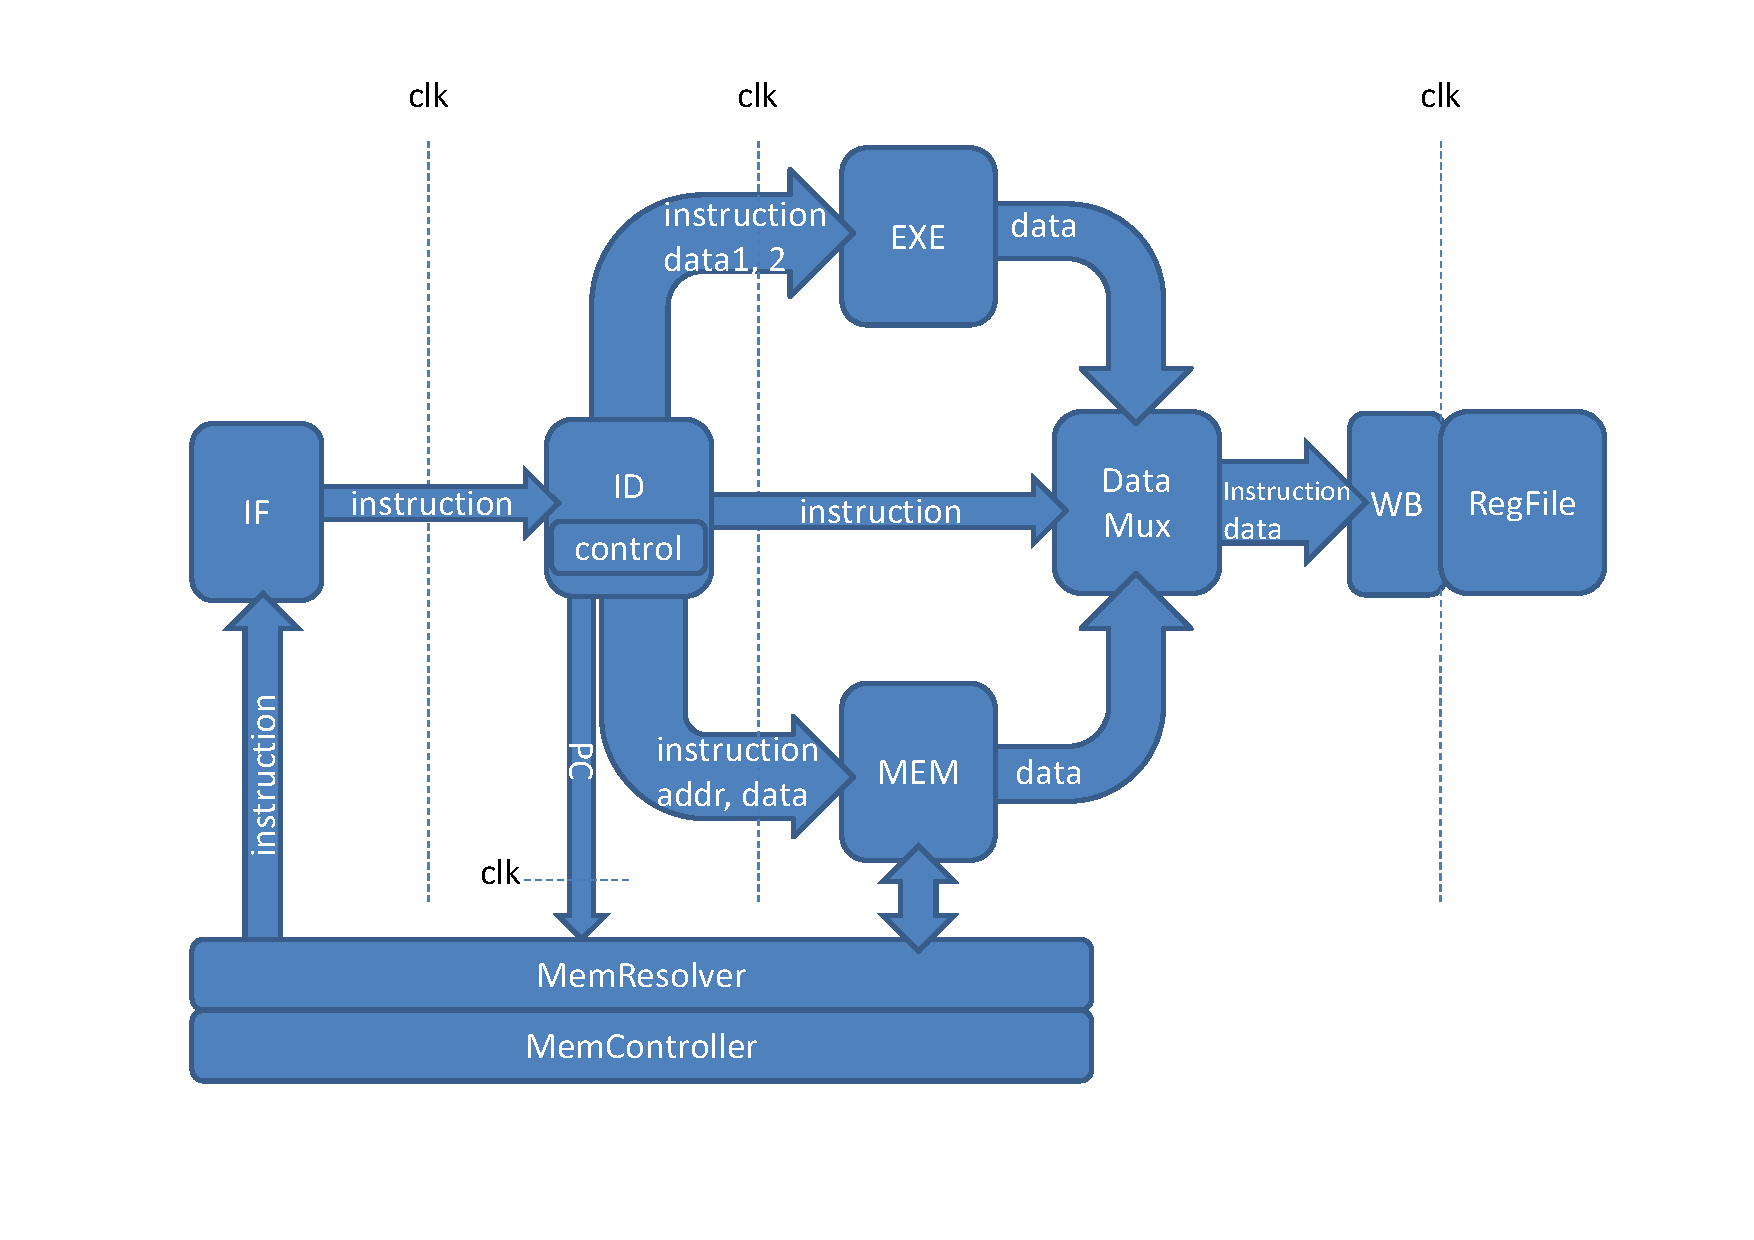
\includegraphics[width=1.0\linewidth]{framework.pdf}

\subsection{模块说明}
\begin{itemize}
\item IF: 从内存获取指令,传输给 ID
\item ID: 包括两个进程\\
1, 对指令做基本的解码,获取相应的寄存器的数据传输给 EXE 和 MEM \\
2, 对控制指令(跳转、中断)等做相应的处理,处理所有的特殊寄存器相关的指令
\item EXE: 进行复杂的计算
\item MEM: 读写内存
\item DataMux: 根据指令来判断选取 EXE 的结果还是 MEM 的结果传输给下一层
\item WB: 根据指令分析得到需要写入的寄存器,并写入到寄存器堆中。
\end{itemize}

\subsection{MEM与EXE并行}
我们对指令集进行了严密的分析,发现内存读写的同时不会伴随复杂的运算,而只是对地址进行简单的加法,这些操作不会占用太多的
时间。所以我们把这两个阶段并行化是十分可行的。具体来说,每条指令都会同时传送给 EXE 和 MEM 两个阶段,这个个阶段再分别
判断自己是否需要处理这个数据,如果需要则进行计算或者进行内存处理,再通过 DataMux 来进行数据选择,将所需数据传给下一阶段。
所以并行化并不会导致每个时钟周期做的事情变多,既可以很好的完成任务,又可以减少整体流水线的复杂度。

\subsection{模块连接}
和其他组不同,我们编写代码时对于 CPU 内部的模块是用 VHDL 代码编写,但是顶层结构我们是利用 Xilinx 的 Schematic 来直接连线完成的。
这样的好处是逻辑清晰,简单明了,同时也省去了顶层组合各个模块的大量代码(许多组的顶层文件都有上百行),避免了人工连接的出错。

schematic 图如下:\\
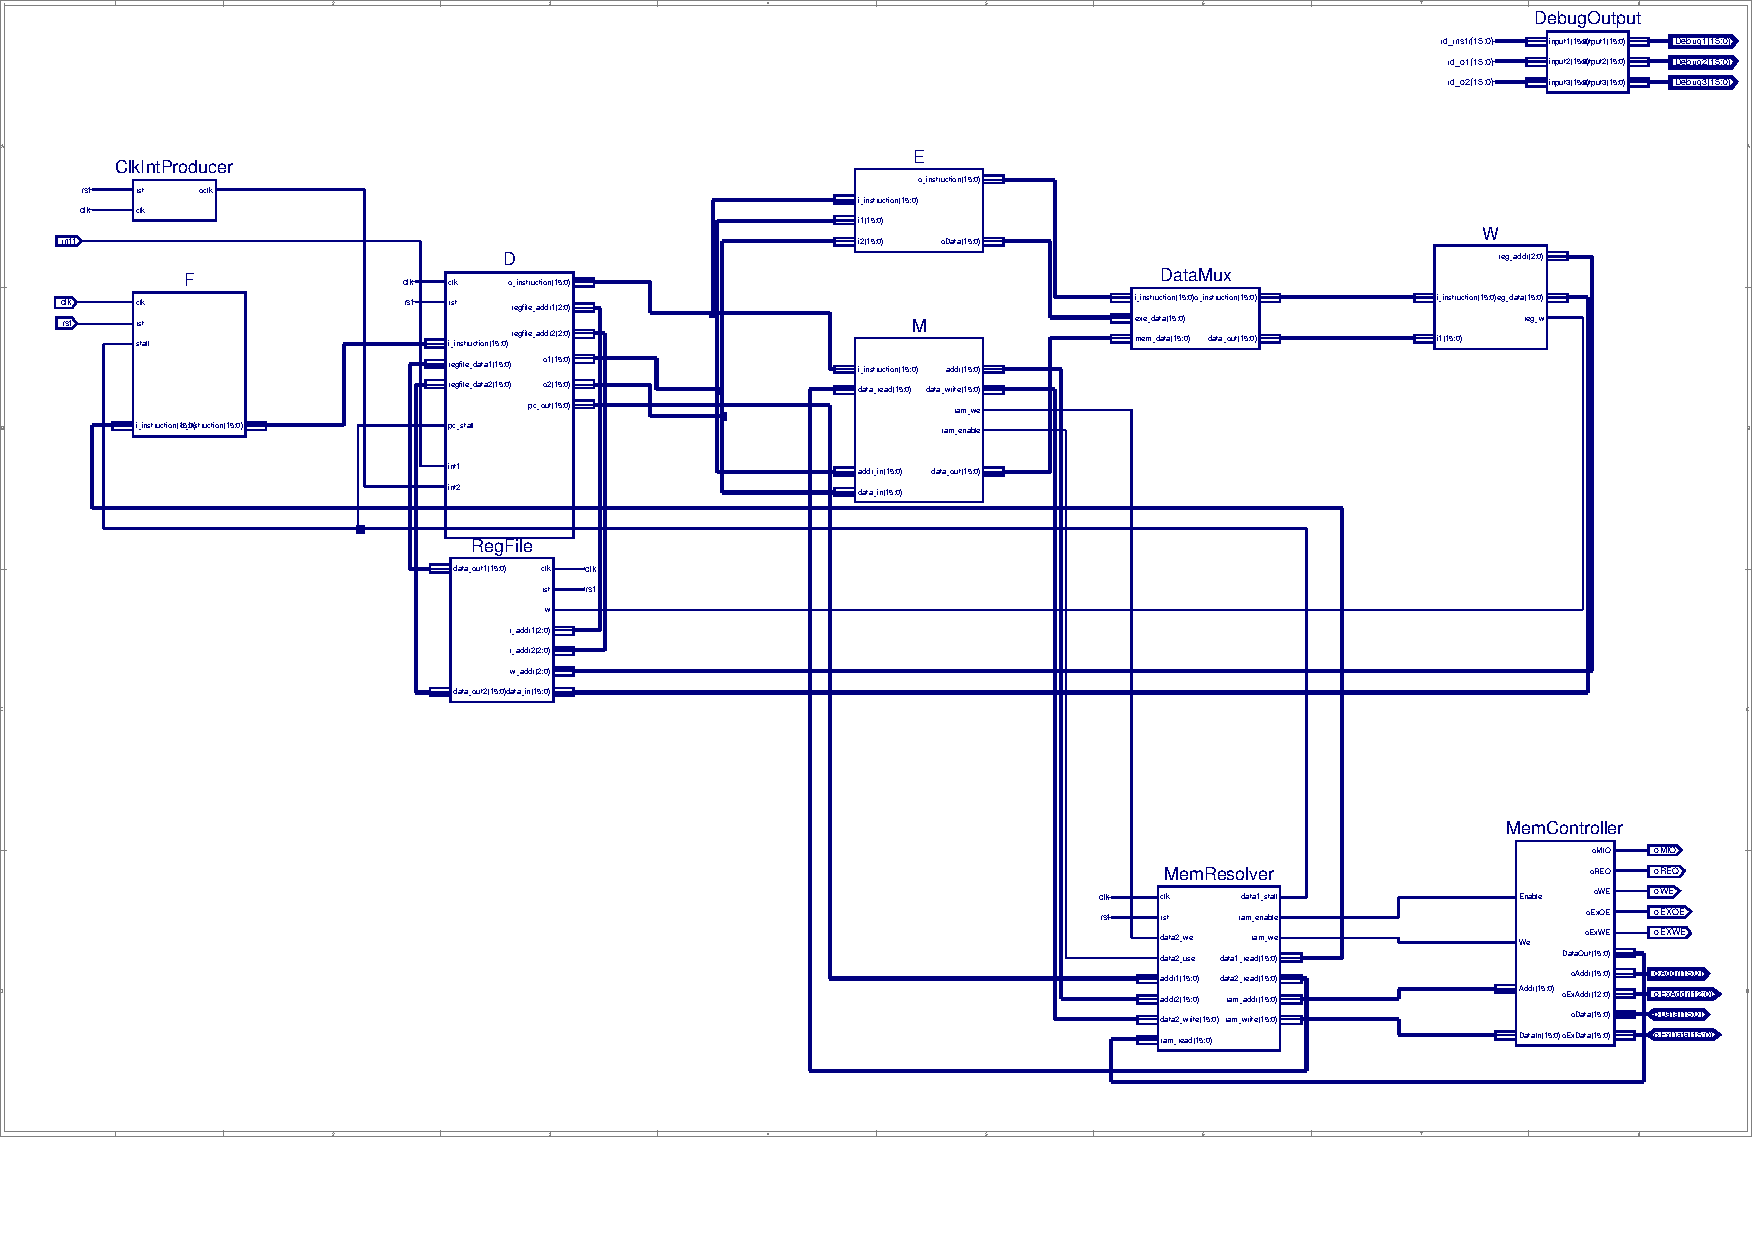
\includegraphics[width=1.0\linewidth]{schematic.pdf}

由图可以清晰地看出我们各个模块的接口,各个模块的联系。

\subsection{RTL图}
下面是由Xilinx软件自动生成的RTL图\\
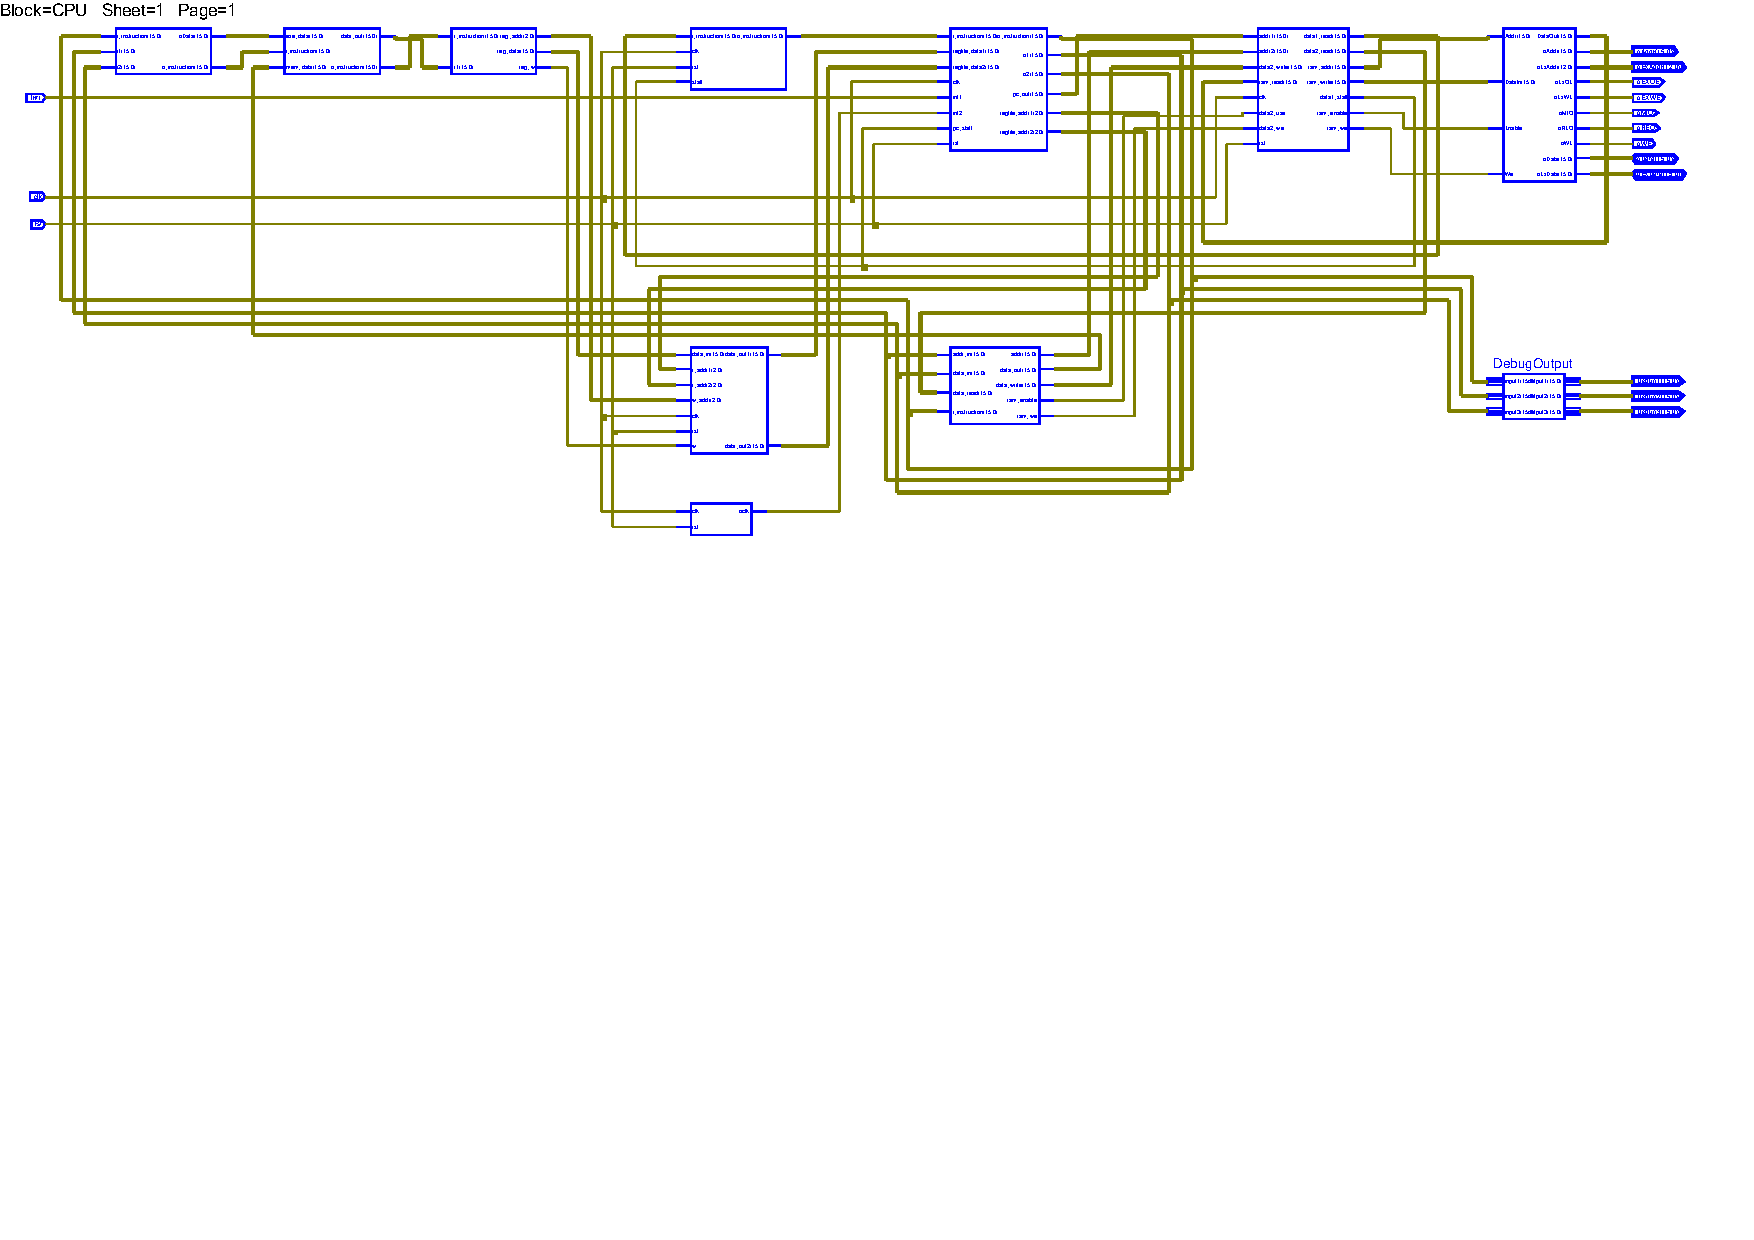
\includegraphics[width=1.0\linewidth,trim=0mm 5cm 0mm 0mm]{rtl.pdf}


\section{模块设计}
\subsection{IF--取指}
IF接口图如下:\\
\begin{center}
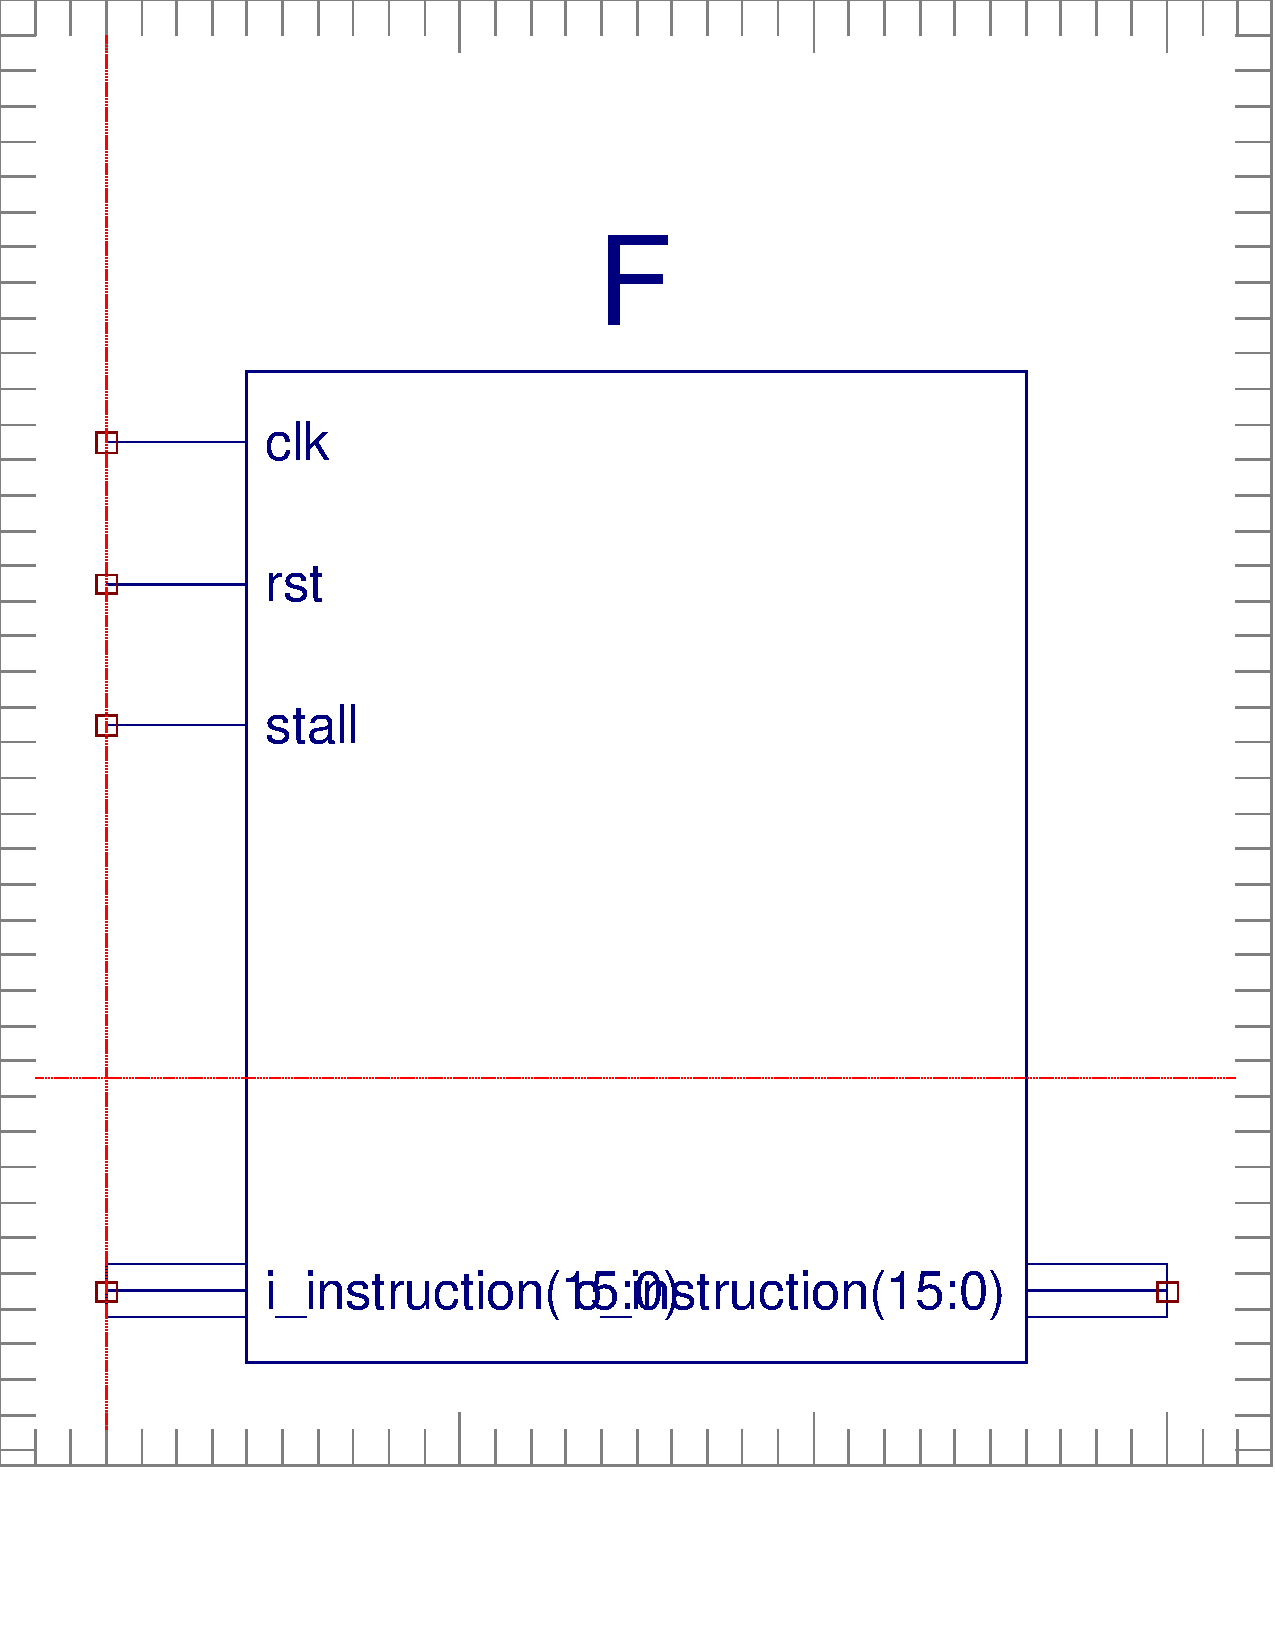
\includegraphics[width=0.5\linewidth]{IF.pdf}
\end{center}

IF是读取指令模块,将指令从内存中取出,传给下一模块ID进行处理,同时接收控制信号,以实现插气泡、中断等功能。
IF的接口定义如下:\\
\begin{center}
\begin{tabular}{|l|l|}\hline
输入&描述\\\hline
clk&时钟信号\\\hline
rst&清零信号\\\hline
stall&锁信号,用于冲突控制\\\hline
i\_instruction&读取的指令\\\hline\hline
输出&描述\\\hline
o\_instruction&输出给下一级的指令\\\hline
\end{tabular}
\end{center}
在 IF 中,若清零或锁信号为1,则将把一条空指令传给下一级,否则才将读取到的指令传给下一级。
IF 读取的指令 i\_instruction 是由 MemResolver 控制的 MemController 读取的,这两个部分将在后面介绍。

\subsection{ID--指令译码}
ID接口图如下:\\
\begin{center}
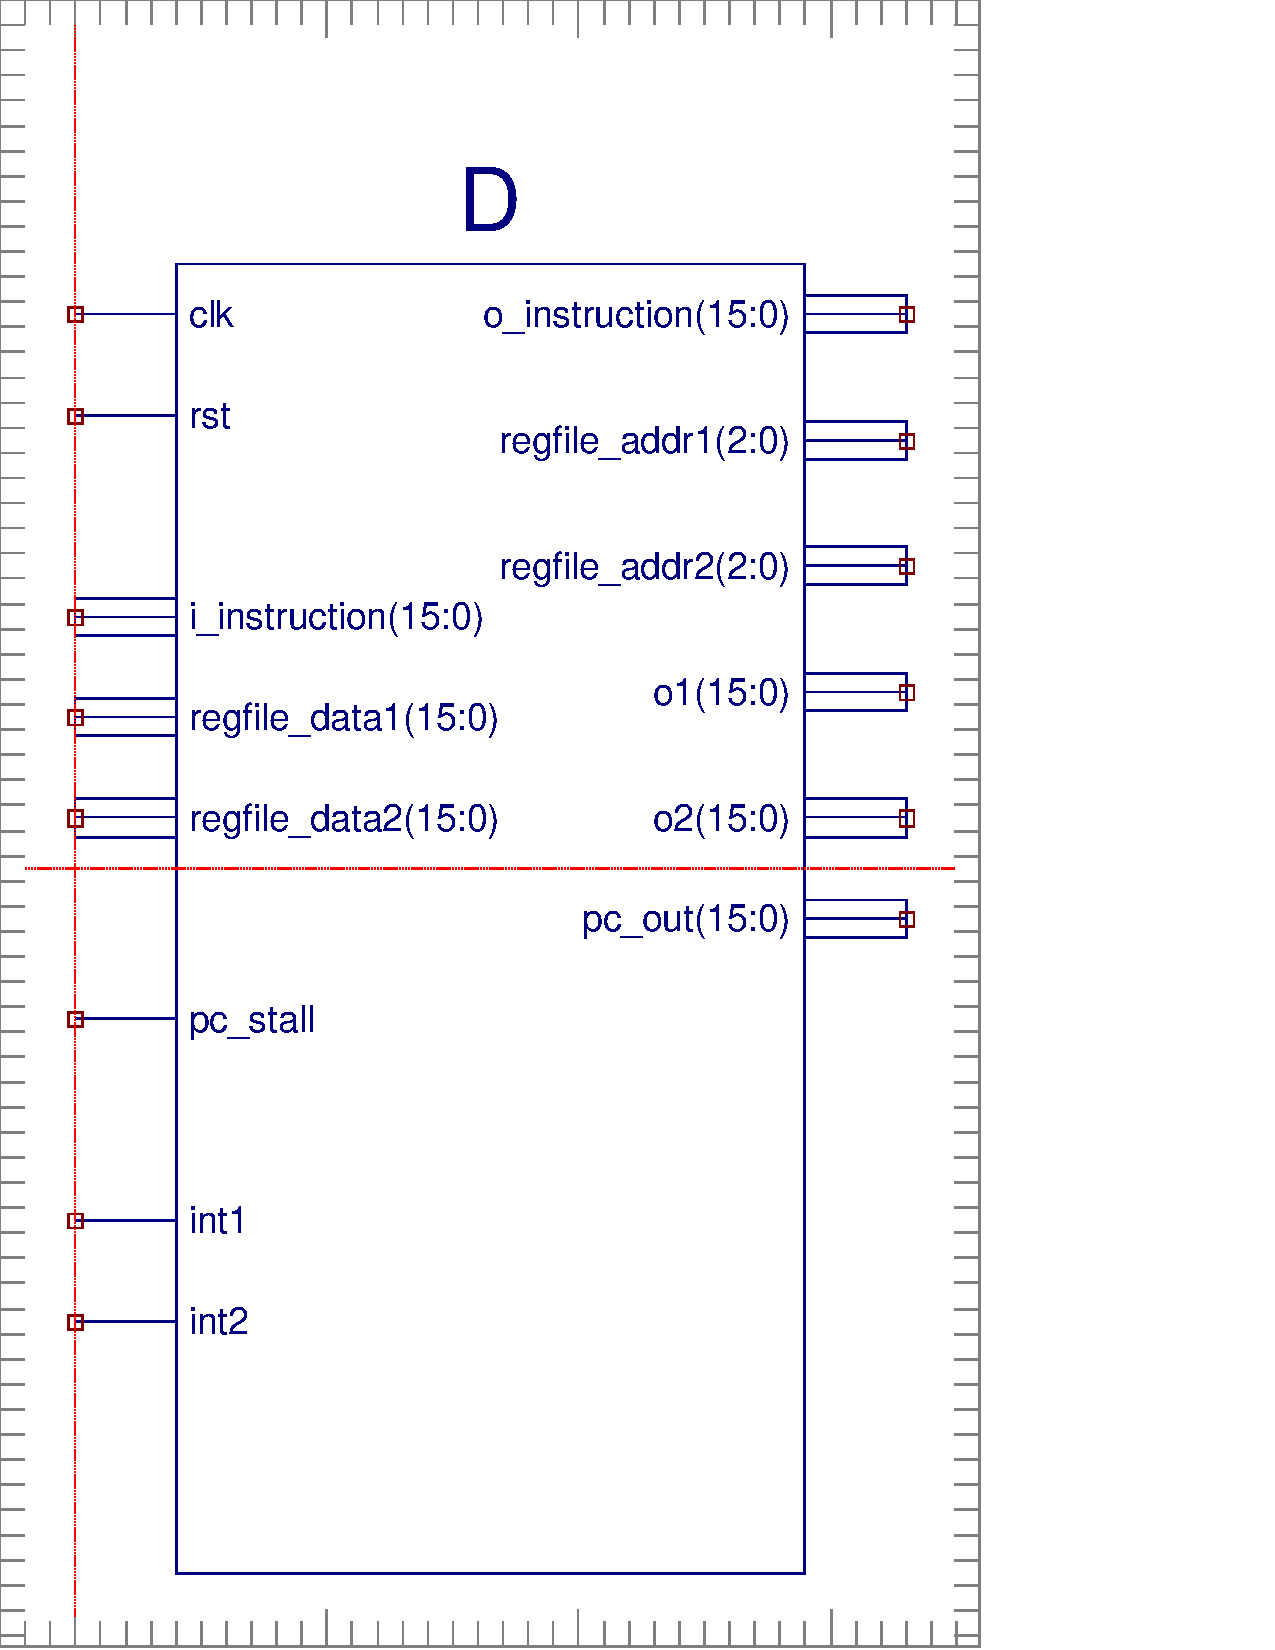
\includegraphics[width=0.5\linewidth]{ID.pdf}
\end{center}
前面已经指出,ID 阶段包括两部分,首先是标准的解码工作,这里的解码工作其实比较简单,主要就是从寄存器堆里面取数据传递给下一
阶段,同时如果指令是内存读写,会进行简单的加法计算需要的地址。

另一部分就是特殊控制部分,这里会处理所有需要特殊寄存器的操作,也就是 SP、IH、RA、T还有PC。这里比较特殊的是  PC 的处理,
也就是所有需要跳转的操作都是在这里完成的,这样做的好处是加上前面IF阶段的延迟,正好是一个延时槽,这样也就免去了分支预测
等的开销,简洁高效。
  
有的同学会认为我们在 ID 阶段做的工作太多了,是不是会导致流水线速度受限,时钟频率无法提高?答案是否定的,我们经过对指令集
的详细分析,和流水线各个线段的认真规划,在严密的考虑下,我们认为已经充分的保证了每个周期工作量的均衡。对 ID 阶段来说,
由于控制进程和解码进程是两个并行的进程,所以总的工作时间不会变长。
实际上我们把控制模块集成到 ID 里面只是为了减少连线的麻烦,两者相对来说是独立的。
   
对于控制模块,处理了所有需要修改特殊寄存器的指令,这也是基于我们对指令集的分析得出的。对特殊寄存器的操作都是比较简单的,
在 ID 阶段完全可以完成。而且对于特殊寄存器的赋值也是在时钟沿之后完成的,进一步减少了 ID 阶段的负担。

ID的接口定义如下:\\
\begin{center}
\begin{tabular}{|l|l|}\hline
输入& 描述\\\hline
clk	&时钟信号\\\hline
rst	&清零信号\\\hline
pc\_stall &暂停信号\\\hline
int1 &硬件中断信号\\\hline
int2 &时钟中断信号\\\hline
i\_instruction	&读取的指令\\\hline
regfile\_data1 &从寄存器堆读取到的数据\\\hline
regfile\_data2 &从寄存器堆读取到的数据\\\hline\hline
输出&描述\\\hline
o\_instruction &指令输出\\\hline
regfile\_addr1 &寄存器地址\\\hline
regfile\_addr2 &寄存器地址\\\hline
o1 &输出给下一级的数据\\\hline
o2 &输出给下一级的数据\\\hline
pc\_out&下一个PC值\\\hline
\end{tabular}
\end{center}

\subsection{EXE--执行}
EXE接口图如下:\\
\begin{center}
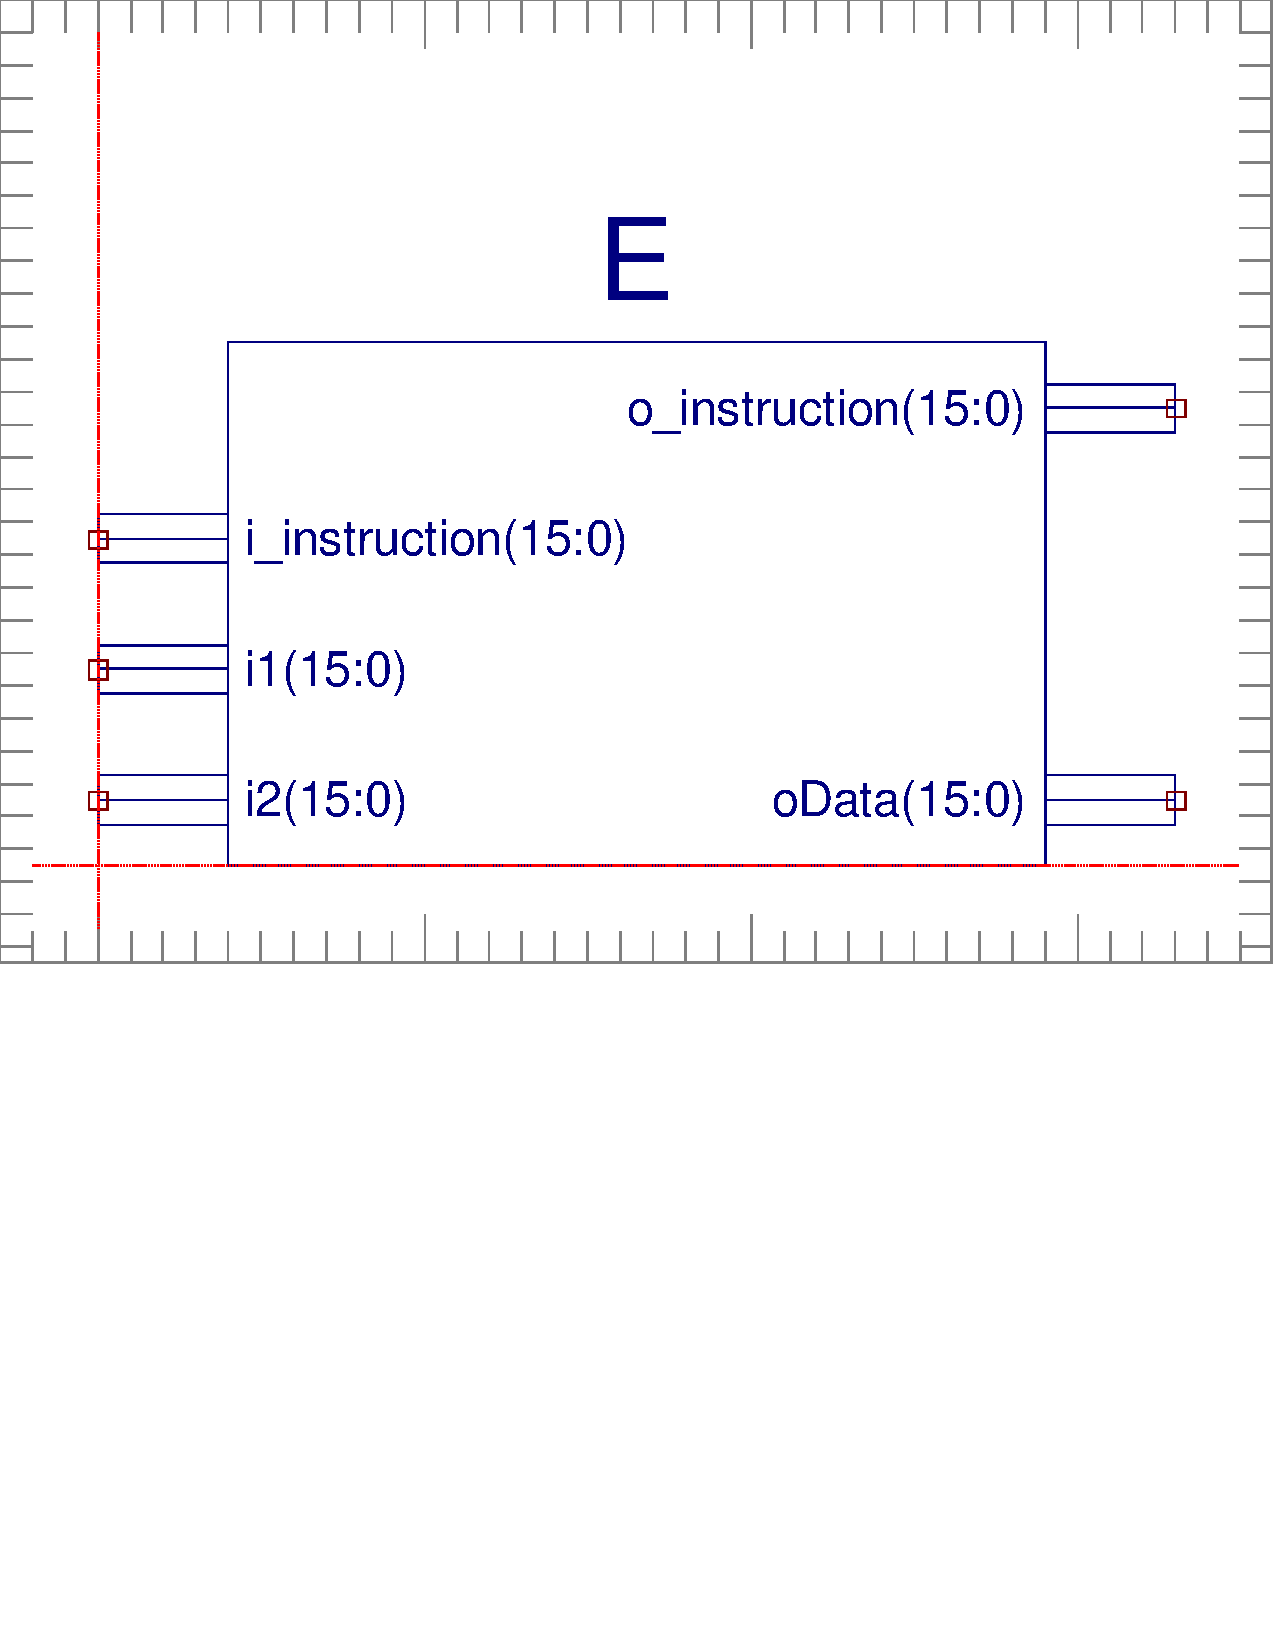
\includegraphics[width=0.5\linewidth,trim=0mm 4cm 0mm 0mm]{EXE.pdf}
\end{center}
运算模块,主要功能是调用 ALU 进行计算,对于不同指令给出对应的 ALU 控制信号和输入数据,并将 ALU 返回的结果传给下一级使用。
IE的接口定义如下:\\
\begin{center}
\begin{tabular}{|l|l|}\hline
输入&描述\\\hline
i\_instruction&输入的指令\\\hline
i1&第一个操作数\\\hline
i2&第二个操作数\\\hline\hline
输出&描述\\\hline
o\_instruction&给下一级的指令\\\hline
oData&\zcell{c}{对当前指令的处理结果,一般为要读取的内存地\\址、写回寄存器的数据等,传给下一级进行处理}\\\hline
\end{tabular}
\end{center}

IE包含的子模块:\\
\begin{itemize}
\item ALU 计算模块
\item Mapper 编码模块
\end{itemize}

IE 根据 Mapper 编码的 op\_link 判断当前为何种指令,并据此给 ALU 不同的输入,给出 alu\_op, alu\_in1, alu\_in2, 其中两个操作数可
能是 ID 模块给出的操作数 i1,i2,也可能是指令中所给的立即数,要从 i\_instruction 中读取,并进行适当的扩展(带符号或无符号);
输出结果 oData 也要根据 op\_link 的不同,可能为 ALU 的输出 alu\_y ,也可能为某一个操作数 i1 或 i2 ,也可能没有值NOVALUE ,
根据情况输出不同的数据给下一级进行处理。

\subsection{ALU--算术逻辑单元}
接口描述:\\
\begin{center}
\begin{tabular}{|l|l|}\hline
输入&描述\\\hline
alu\_op&给ALU的控制码,指示ALU进行何种运算\\\hline
alu\_in1&操作数1\\\hline
alu\_in2&操作数2\\\hline
alu\_cin&进位输入\\\hline\hline
输出&描述\\\hline
alu\_y&输出结果\\\hline
alu\_c&输出进位标志位\\\hline
alu\_z&输出零标志位\\\hline
\end{tabular}
\end{center}


\subsection{MEM--访存}
MEM接口图如下:\\
\begin{center}
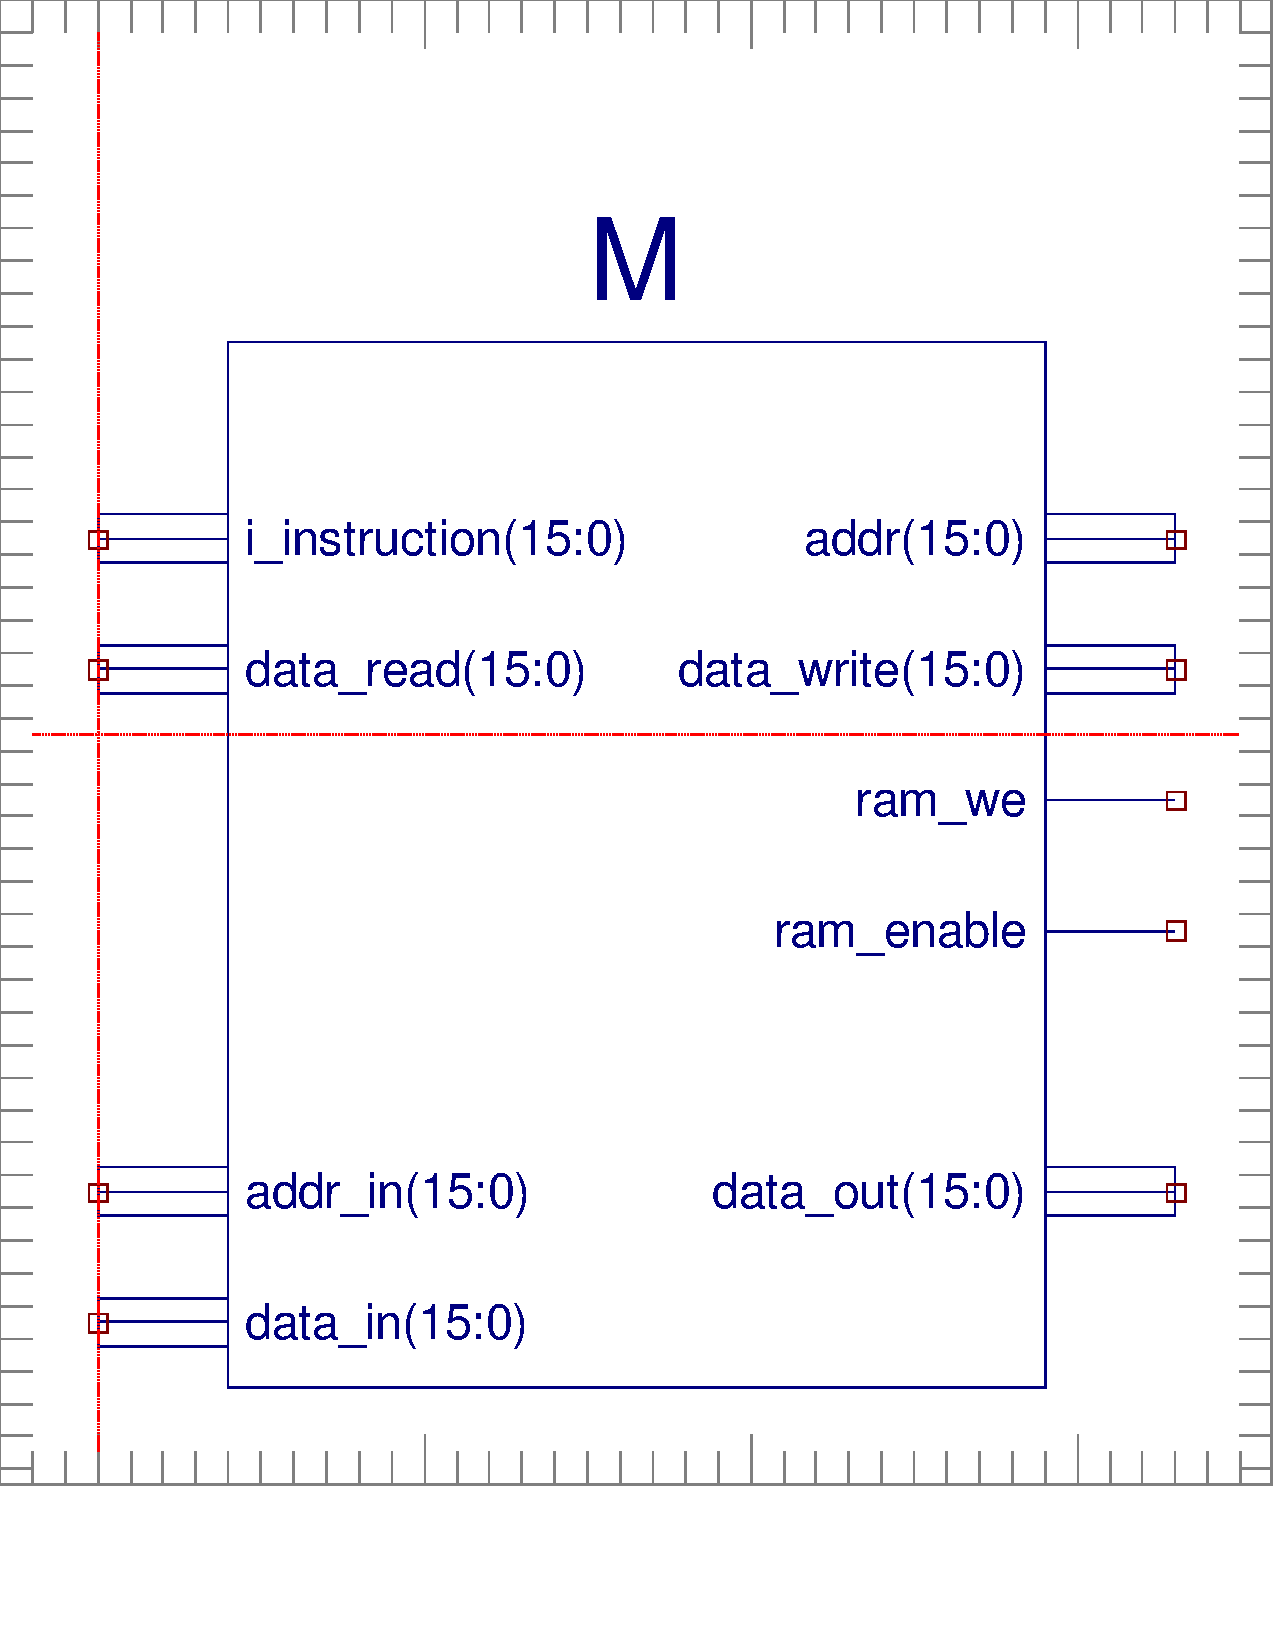
\includegraphics[width=0.5\linewidth]{MEM.pdf}
\end{center}
访存模块,实现对内存 RAM 的读写。实际的对内存的控制是由 MemController, MemResolver 实现的,MEM 模块实际上只是给这两个模块发出
内存读写的控制信号,并为上下级传递读写的数据。\\
MEM 的接口定义如下:\\
\begin{center}
\begin{tabular}{|l|l|}\hline
输入&描述\\\hline
i\_instruction&从上一级读取到的指令\\\hline
addr\_in&从ID模块传来的地址\\\hline
data\_in&从ID模块传来的数据\\\hline
data\_read&从MemResolver,MemController读取的内存数据\\\hline\hline
输出&描述\\\hline
data\_out& 给下一级的数据\\\hline
addr&给MemResolver的地址\\\hline
data\_write& 要写入内存的数据\\\hline
ram\_we&写使能\\\hline
ram\_enable&使用Mem信号\\\hline
\end{tabular}
\end{center}

包含的子模块:\\
Mapper\\
MEM根据从Mapper得到的 op\_link 设置 ram\_enable,ram\_we, 并将访问的数据传递给下一级。

\subsection{WB--写回}
WB接口图如下:\\
\begin{center}
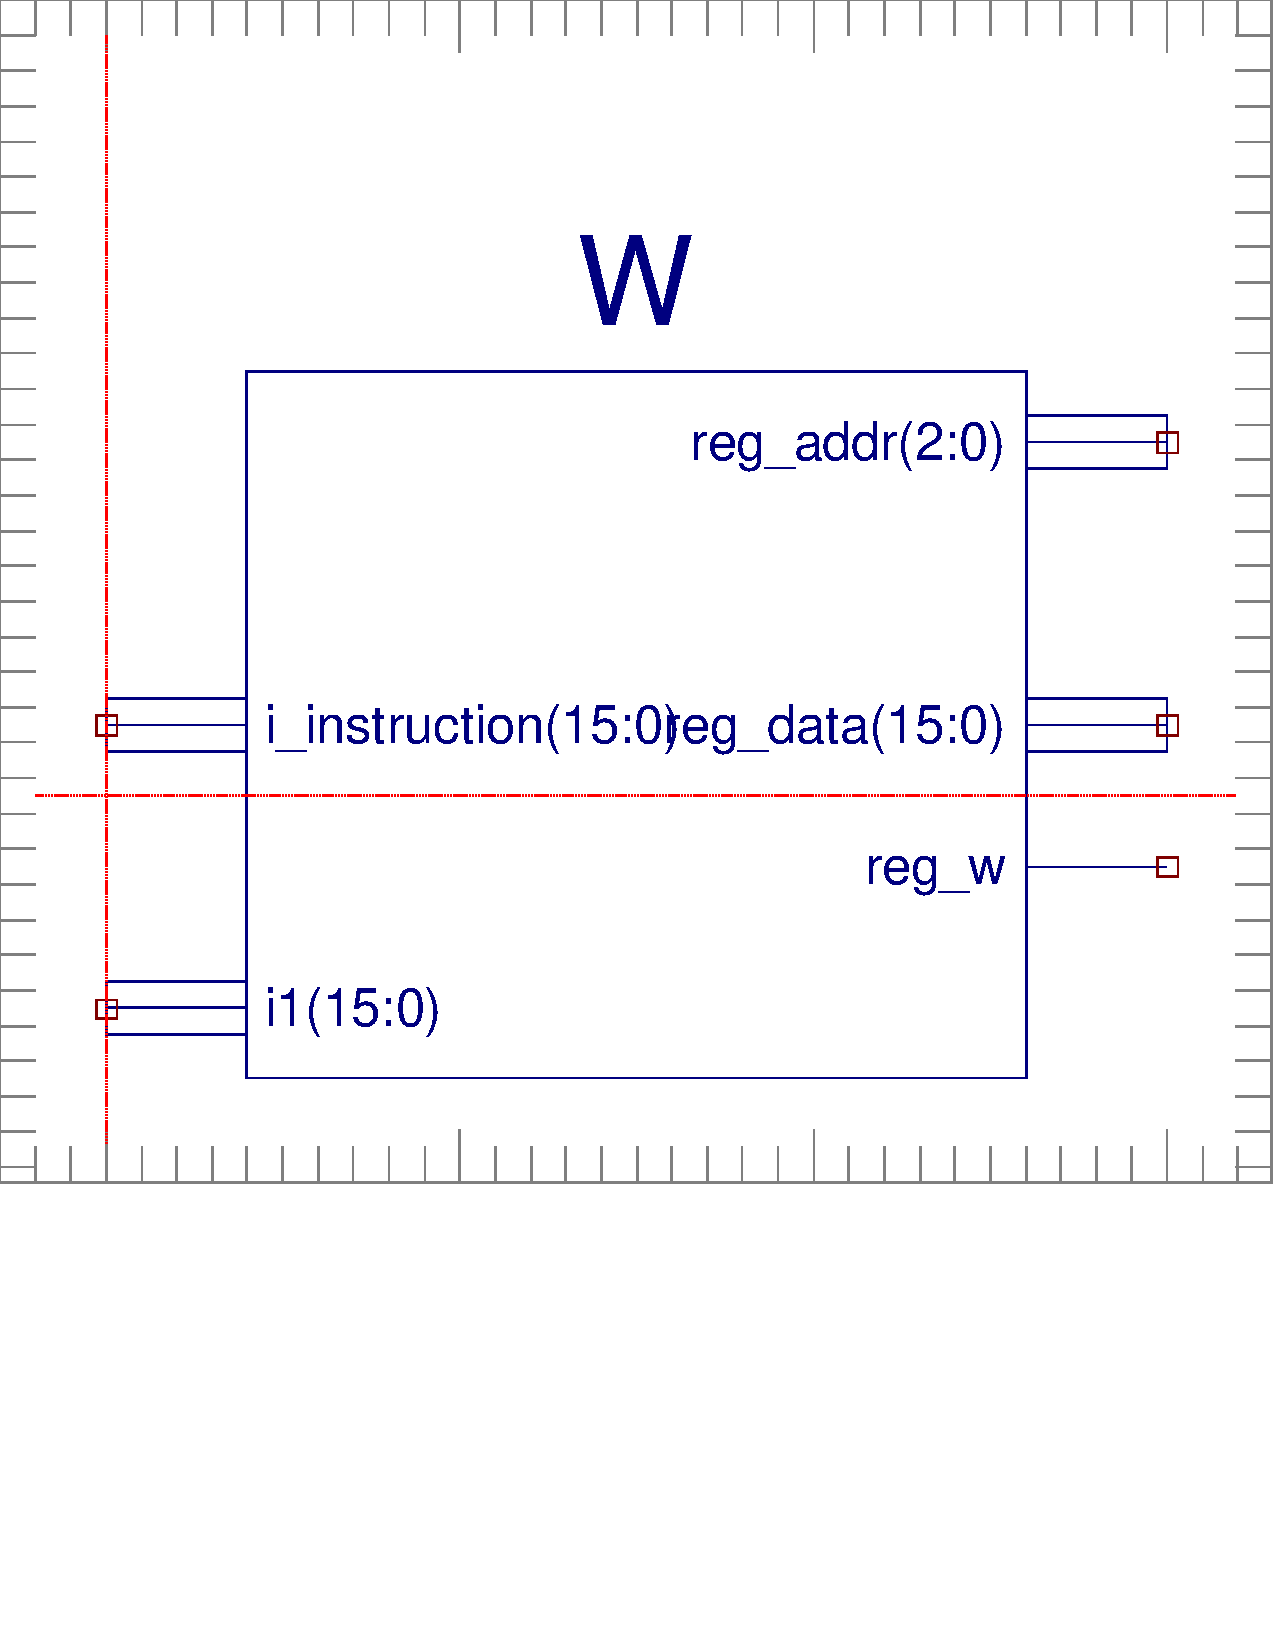
\includegraphics[width=0.5\linewidth]{WB.pdf}
\end{center}
WB 是写回寄存器模块,将 IE 或 MEM 所给的数据写回数据寄存器。通过 Mapper 得到的 op\_link 判断要写回的寄存器,从 i\_instruction 
中取出相应的寄存器 reg\_addr ,将数据写入寄存器。\\
WB的接口定义如下:\\
\begin{center}
\begin{tabular}{|l|l|}\hline
输入&描述\\\hline
i\_instruction&从DataMux传来的指令\\\hline
i1&DataMux的数据\\\hline\hline
输出&描述\\\hline
reg\_addr&输出给寄存器堆的地址\\\hline
reg\_data&输出给寄存器堆的舒适\\\hline
reg\_w&是否写寄存器堆\\\hline
\end{tabular}
\end{center}

\subsection{MemResolver--内存访问冲突控制器}
MemResolver接口图如下:\\
\begin{center}
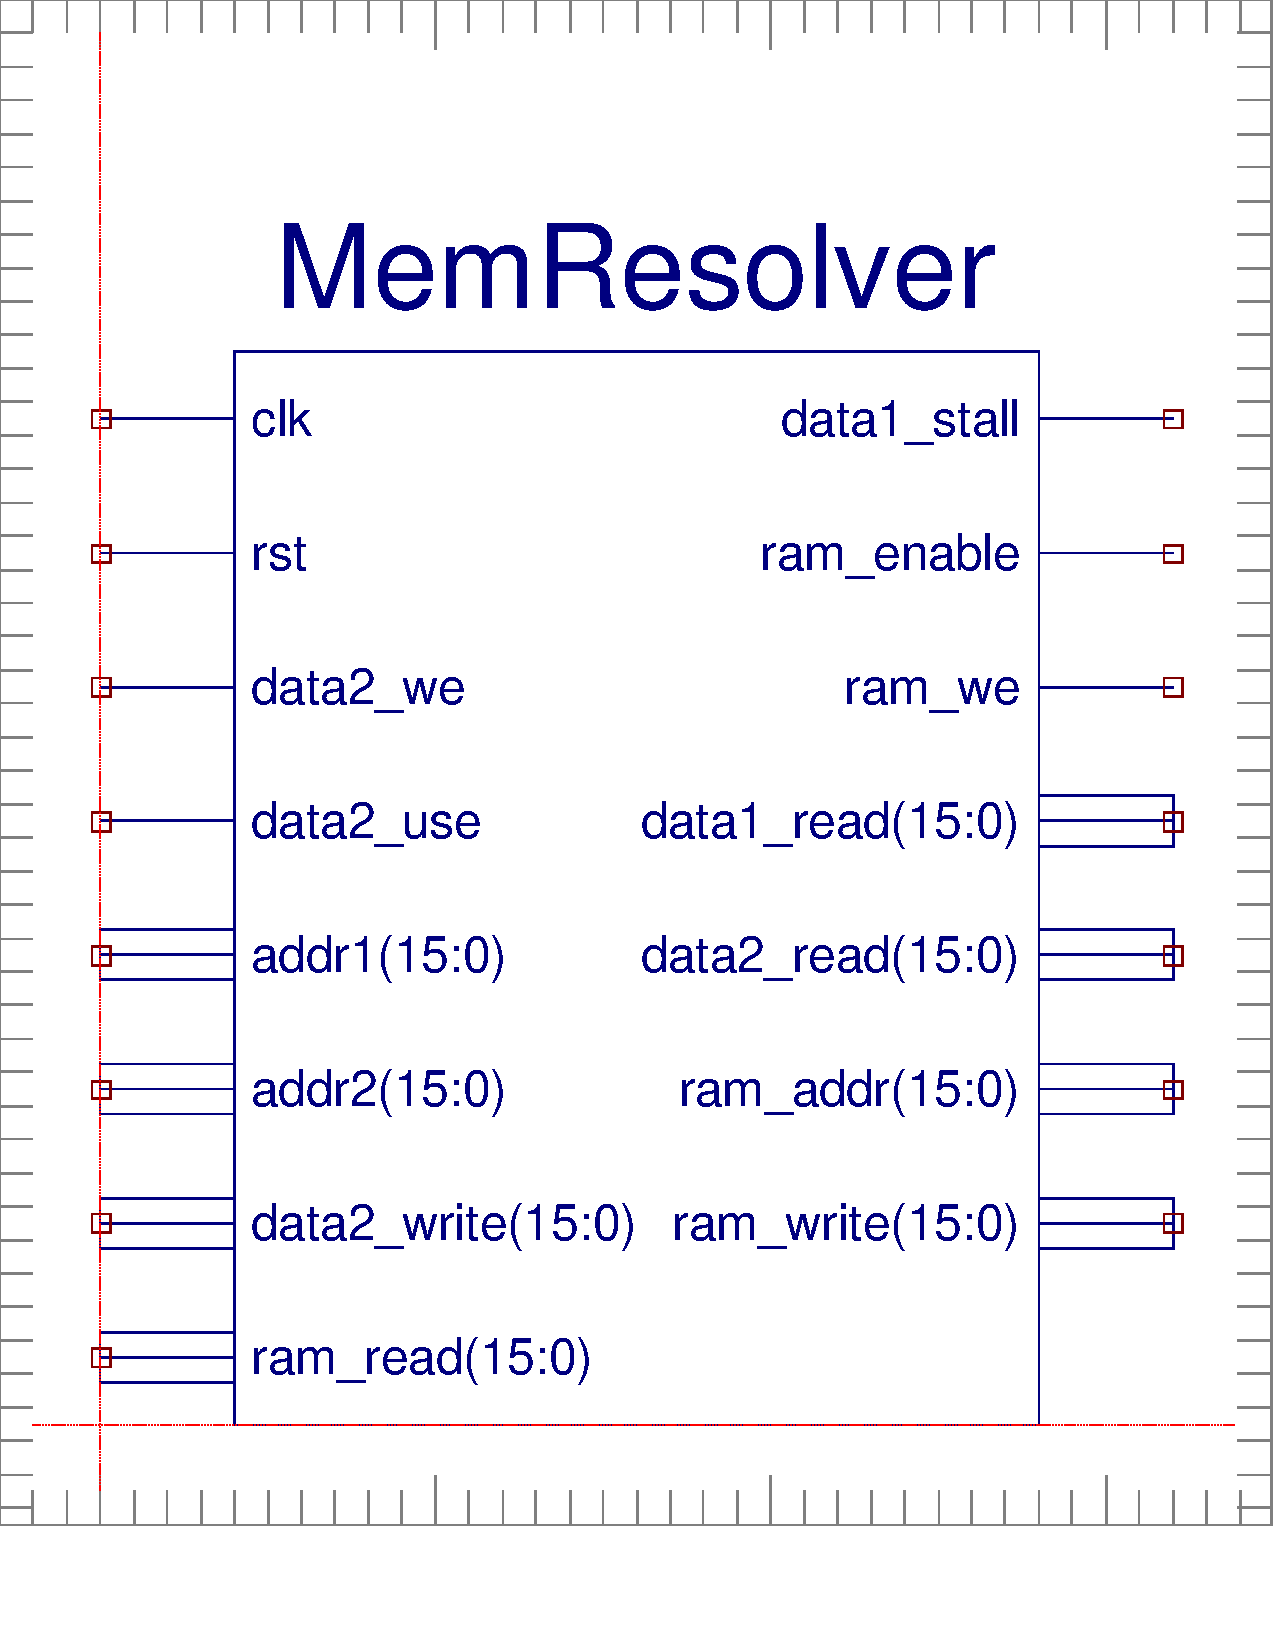
\includegraphics[width=0.5\linewidth]{MemResolver.pdf}
\end{center}
由于 IF 阶段和 MEM 阶段都需要读取内存,而 MemController 只能实现一个周期读取一条指令,并且也只有一个接口,因此我们设计了
MemResolver ,他接收 IF 和 Mem 两个模块的内存访问要求,同时做他们的冲突控制(如果二者同时需要访问就给 IF 和 ID 一个暂停信号)。

另外,Cache 也是实现在 MemResolver 中的,对于每一个读访问, MemResolver 会先从 Cache 中试着读取数据,如果没有找到再去访问内存。

MemResolver的接口定义如下:\\
\begin{center}
\begin{tabular}{|l|l|}\hline
输入&描述\\\hline
clk&时钟信号\\\hline
rst&复位信号\\\hline
data2\_we&MEM模块的写使能\\\hline
data2\_use&MEM模块的使用信号\\\hline
addr1&ID模块给出的地址\\\hline
addr2&MEM模块给出的地址\\\hline
data2\_write&MEM模块的写数据\\\hline
ram\_read&从内存中读取到的数据\\\hline\hline
输出&描述\\\hline
data1\_still&当读取内存冲突时给ID的暂停信号\\\hline
ram\_enable&给MemController的使能信号\\\hline
ram\_we&给MemController的写使能\\\hline
data1\_read&读取到的数据送给ID模块\\\hline
data2\_read&读取到的数据送给MEM模块\\\hline
ram\_addr&给MemController的地址\\\hline
ram\_write&给MemController的写数据\\\hline
\end{tabular}
\end{center}

\subsection{MemController--内存访问控制}
MemController接口图如下:\\
\begin{center}
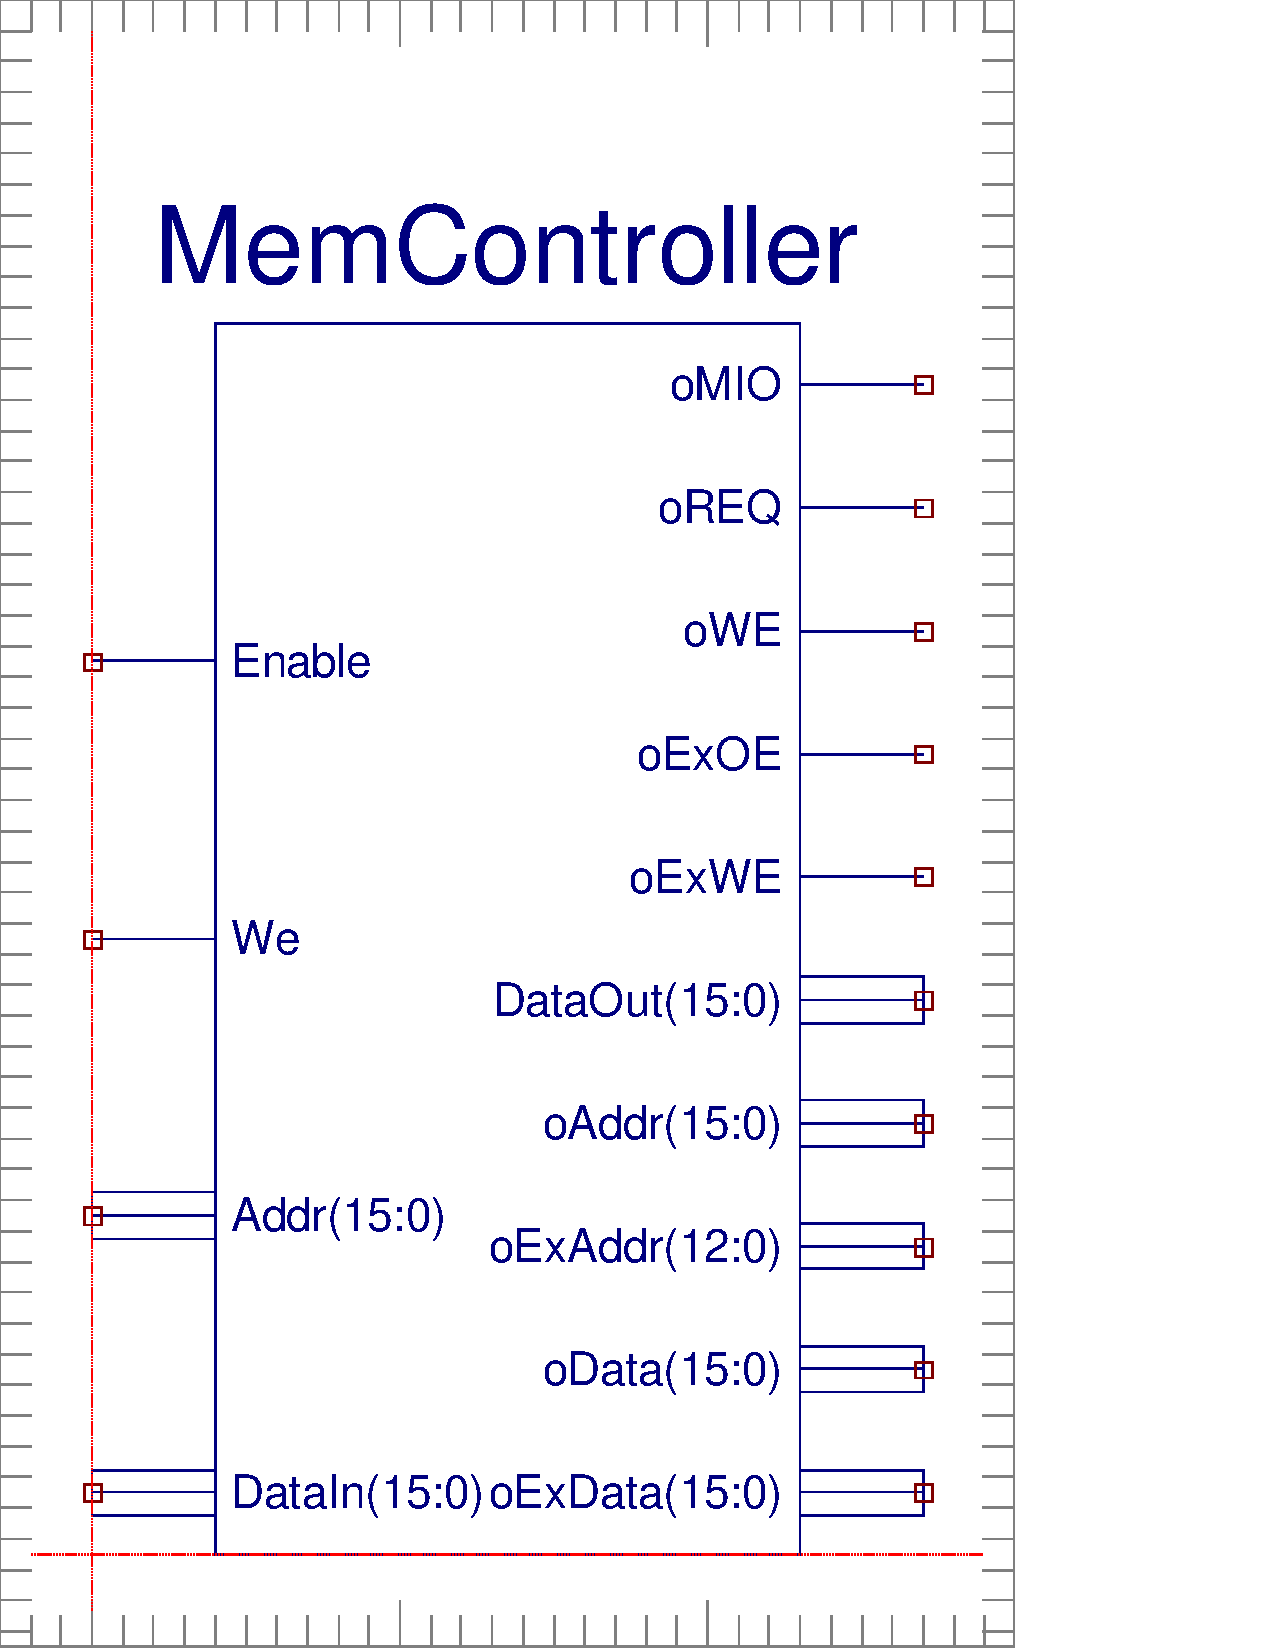
\includegraphics[width=0.5\linewidth]{MemController.pdf}
\end{center}
MemController 是内存访问的控制器,它接收访问地址,数据和写的信号,然后通过地址映射来与基本  ROM ,基本 RAM ,扩展 RAM 和串口
通信。所以他通过封装向上提供了一个统一的内存访问接口,方便了上层的内存交互。

MemController的接口定义如下:\\
\begin{center}
\begin{tabular}{|l|l|}\hline
输入&描述\\\hline
Enable&使能信号\\\hline
we&写使能信号\\\hline
addr&地址信号\\\hline
datain&写数据\\\hline\hline
输出&描述\\\hline
oMIO&控制信号,MIO\\\hline
oREQ&控制信号,REQ\\\hline
oWE&控制信号,WE写使能\\\hline
oExOE&控制信号,扩展ram输出使能\\\hline
oExWE&控制信号,扩展ram写使能\\\hline
oAddr&地址线\\\hline
oExAddr&扩展地址线\\\hline
oData&要写到基本内存的数据\\\hline
oExData&要写到扩展内存的数据\\\hline
\end{tabular}
\end{center}

\subsection{Mapper--指令映射}
在 CPU 内部,我们用一个 integer 为指令编号,Mapper 的作用就是把一条指令映射成其相对应的指令编号。为了便于指令处理,实现简单,
我们在给指令编号的时候专门做了分类优化,按照指令使用的寄存器数进行分类整理,给编码和除错都带来了极大的便捷。
其接口定义如下:\\
\begin{center}
\begin{tabular}{|c|c|}\hline
输入&描述\\\hline
i\_instruction&当前指令\\\hline\hline
输出&描述\\\hline
op\_link&转换后的编码,通过此编码可以知道当前指令为何指令\\\hline
\end{tabular}
\end{center}

指令分类优化表见附录1。

\subsection{RegFile--寄存器堆}
RegFile接口图如下:\\
\begin{center}
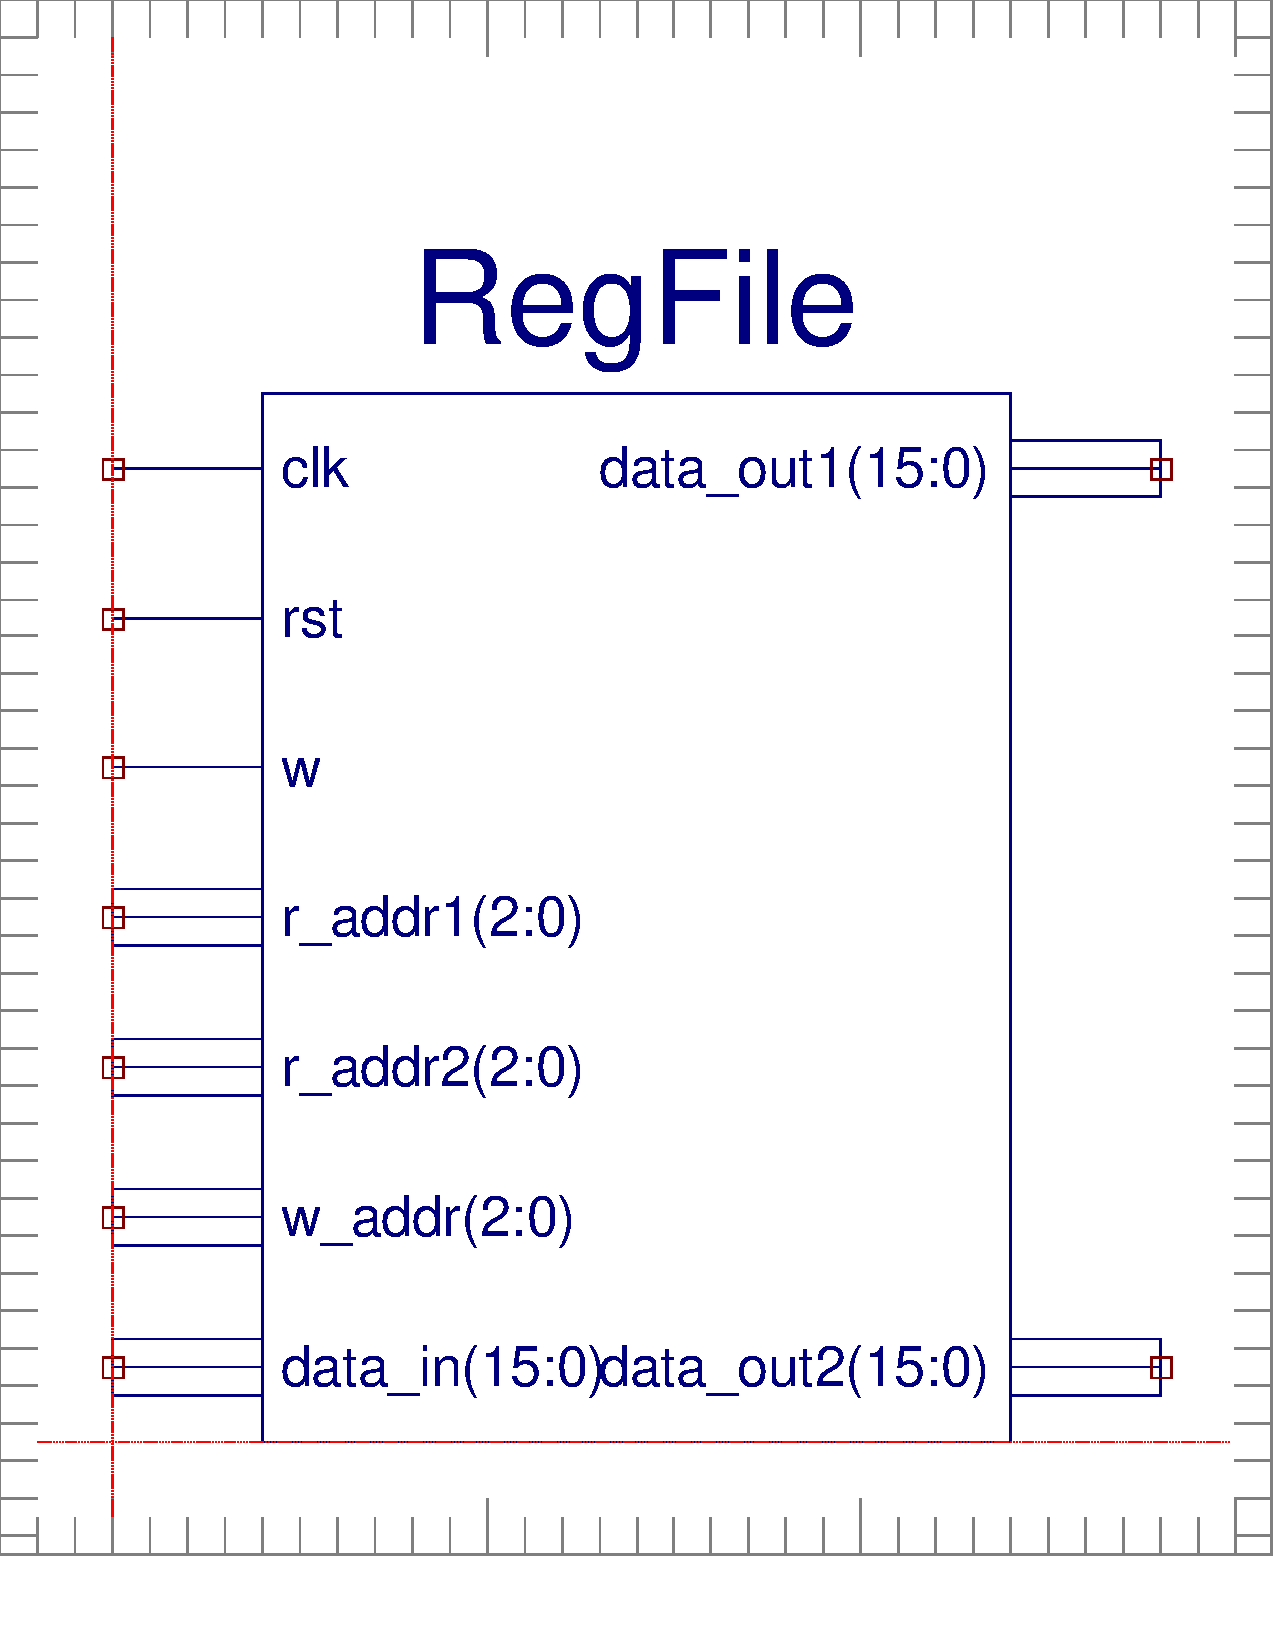
\includegraphics[width=0.5\linewidth]{regfile.pdf}
\end{center}

寄存器堆里面是 R0-R7, 总共8个16位通用寄存器。他提供一路写(由WB来写),两路读(都是给ID),通过地址来访问数据。对于寄存器堆的
操作,读取的时候它是组合逻辑,保证当前时钟周期就能拿到数据,而对于写入操作,是时序逻辑,时钟周期过后才能把数据写入。

另外,数据旁路的实现也在 RegFile 中,这个在后面扩展部分会有详细叙述。

其接口定义如下:\\
\begin{center}
\begin{tabular}{|c|c|}\hline
输入&描述\\\hline
clk&时钟信号\\\hline
rst&复位信号\\\hline
w&写信号,表明是否写\\\hline
r\_addr1&读取地址1\\\hline
r\_addr2&读取地址2\\\hline
w\_addr&写入地址\\\hline
data\_in&写入的数据\\\hline\hline
输出&描述\\\hline
data\_out1&数据输出1\\\hline
data\_out2&数据输出2\\\hline
\end{tabular}
\end{center}

\subsection{特殊寄存器}
特殊寄存器不是一个单独的模块,为了操作上面的方面,我们所有的特殊寄存器都是以 signal 的形式放在了 ID 模块里,包括
pc(cur\_pc),SP,RA,IH,T.
由于对这些寄存器的操作在 ID 阶段都已经有能力完全处理,因此他们的操作都放在了ID模块中。

虽然表明上看来这样有些混乱,比如
CMP 指令需要更新T寄存器,那么就需要在 ID 阶段做 CMP 操作,但是事实证明,这样的设计不仅可行,而且会大大简化代码。首先,对于
特殊寄存器的所有数据冲突都不存在,因为每个指令需要的特殊寄存器数据在上个周期就已经被写入了,这样就不需要对于特殊寄存器
的数据旁路了,其次,把特殊寄存器放在 ID 里,使各种和特殊寄存器相关的操作都变简单了,他们只需直接读取和改写即可,
不需要再向其他模块发送地址,读取信号等,也没有任何冲突需要处理。

\subsection{DataMux--数据选择器}
数据选择器是一个简单的组合逻辑,它放在 EXE ,MEM 和 WB 模块之间, 作用是根据指令的不同选择 MEM 和 EXE 中的一个结果传给 WB 阶段。
DataMux接口图如下:\\
\begin{center}
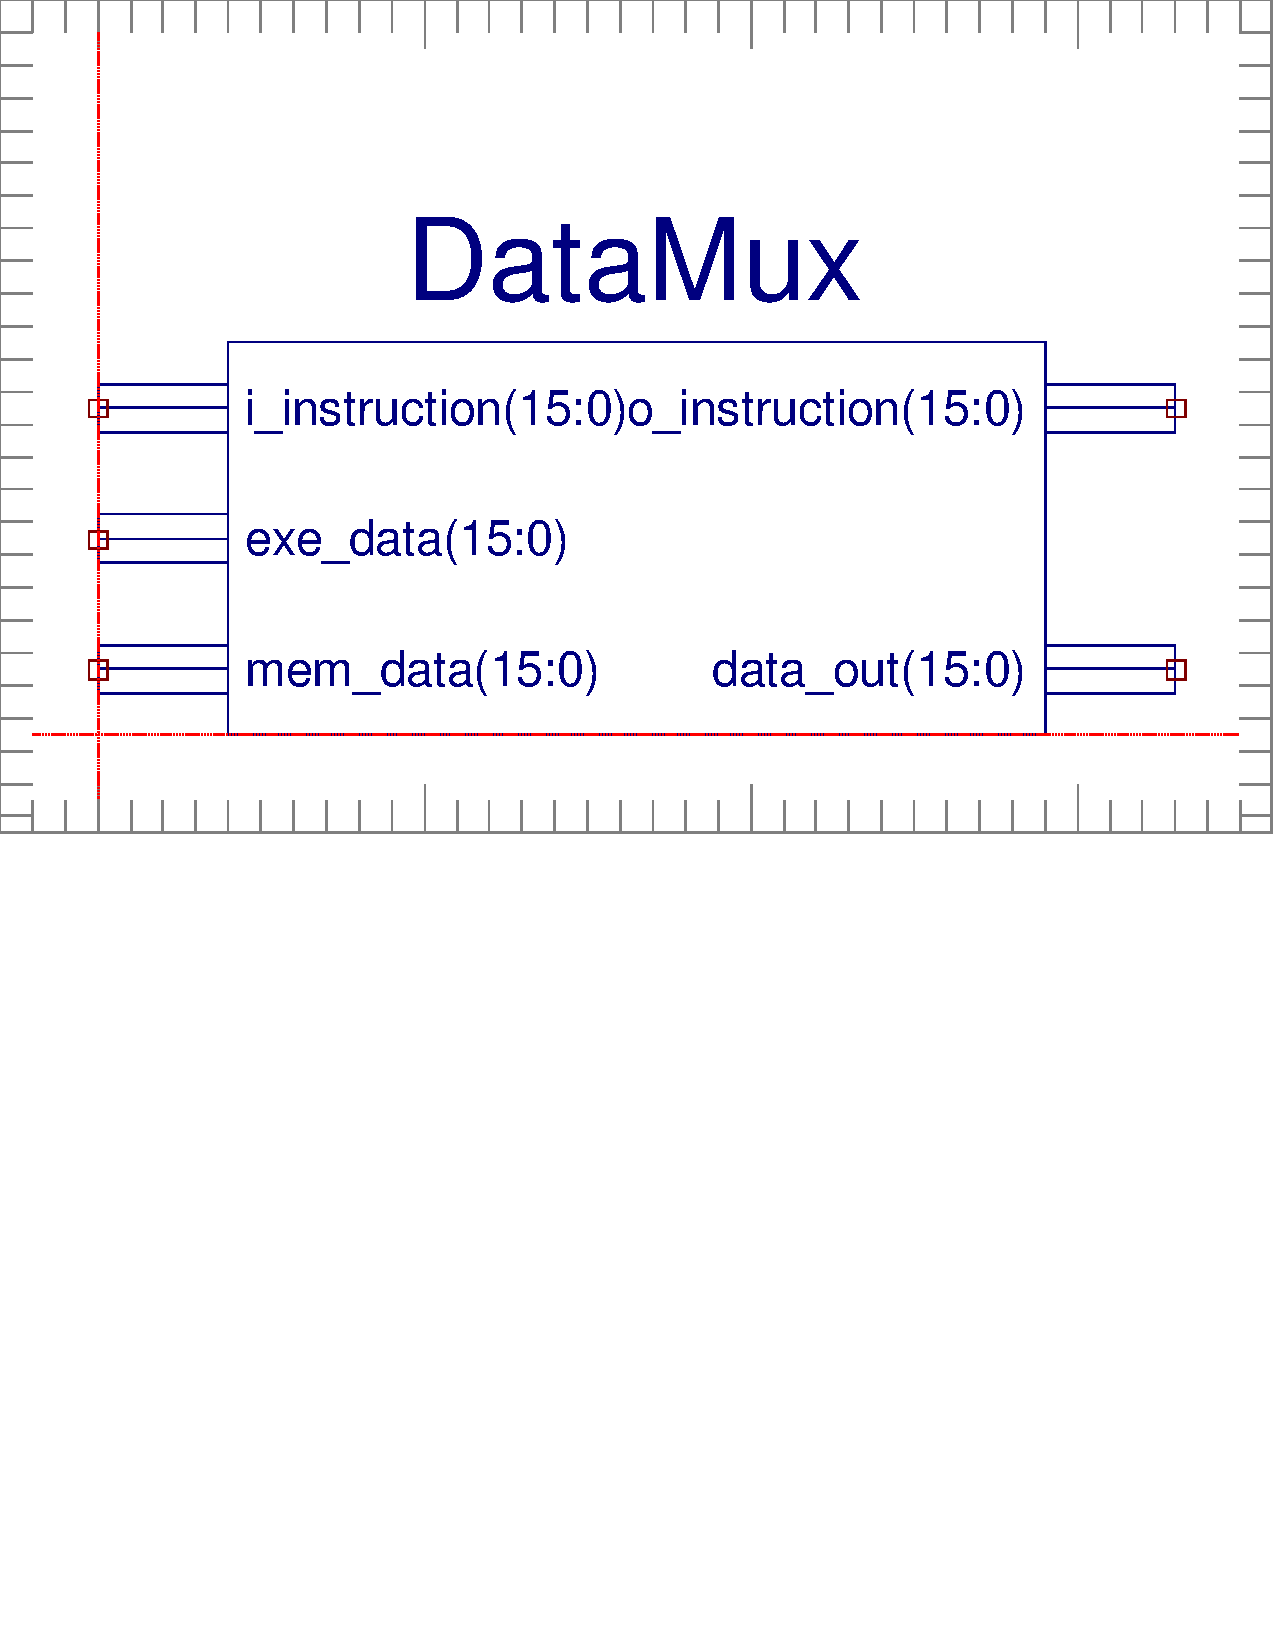
\includegraphics[width=0.5\linewidth,trim=0mm 5cm 0mm 0mm]{datamux.pdf}
\end{center}

其接口定义如下:\\
\begin{center}
\begin{tabular}{|c|c|}\hline
输入&描述\\\hline
i\_instruction&当前指令\\\hline
mem\_data&MEM模块传入的数据\\\hline
exe\_data&EXE模块传入的数据\\\hline\hline
输出&描述\\\hline
o\_instruction&当前指令输出\\\hline
data\_out&数据输出\\\hline
\end{tabular}
\end{center}

\subsection{ClkIntProducer--时钟中断信号产出}
ClkIntProducer 的作用是产生时钟中断信号,为实现时钟中断设立的。实际上它是一个分频器,将 clk 信号分频来产生时钟中断。
目前我们的设置是每10000个时钟产生一次时钟中断信号。

\subsection{DebugOutput--调试输出}
DebugOutput 是我们的调试输出模块,它提供三路16位输入,然后分别将结果输出到 TEC 2008 右上角的 48 个灯上,这为我们调试代码
提供了极大的方便。由于 ID 阶段比较重要,处理的事情也比较多,我们将 DebugOutput 的输入接在了 ID 模块的输出上,这样可以很方便
的看到每一条指令的处理情况。

\section{扩展内容}
\subsection{延时槽}
\subsubsection{概述}
延迟槽的实现比较自然。ID 模块的 pc\_out 给出下一个 pc 值,并交给 MemResolver 去取指令,取到的指令会交给 IF,然后再过一个周期之后,
指令就会传到 ID。这样遇到一条跳转指令的时候,它的下一条指令实际上已经取出来到 IF 中了,然后就会传给 ID 及以后的阶段,从而实现
了延时槽。

\subsubsection{延时槽指令分析}
下面举一个例子来说明延时槽中的指令是如何被执行的.\\
假设指令序列及其 PC 值如下:\\
\begin{center}
\begin{tabular}{|c|l|}\hline
PC & Instruction \\\hline
1  & LI R0 0\\\hline
2  & JR R7  \\\hline
3  & LI R1 1\\\hline
\end{tabular}
\end{center}

当指令1处在 ID 阶段的时候,指令2处在 IF 阶段,这个时候 ID 里面的 cur\_PC 值为1,next\_PC 值为2,当时钟周期来的时候,next\_PC 变为3
并输出给 MemResolver 去取指令3,cur\_PC 变为2,JR R7指令到达 ID 阶段,同时指令3被取出到达 IF 阶段。这样再来一个时钟周期的时候,
指令3就会进入 ID 阶段并一直执行下去,从而完成了延时槽。

以上过程列表如下:\\
\begin{center}
\begin{tabular}{|c|c|c|c|c|}\hline
IF & \multicolumn{4}{|c|}{ID}\\\hline
指令&指令&cur\_PC&next\_PC&pc\_out\\\hline
JR R7&LI R0 0&1&2&3\\\hline
LI R1 1&JR R7&2&3&R7\\\hline
\end{tabular}
\end{center}


\subsection{数据旁路}
\subsubsection{概述}
由于在我们的设计中,WB 阶段和 ID 阶段之间只有一个周期的空白,因此对于写后读冲突来说,要读的数据和要写的数据最多只有一个周期
的距离,所以我们只需要处理一级数据冲突。又因为只有一个周期的距离,因此发生冲突的时候他们会同时对同一个寄存器堆同一地址
进行读和写,这时,只要把要写的数据返回给读取者,这样就实现了数据旁路。

\subsubsection{实现方法}
根据前面的叙述,实现数据通路的方法变得非常简单,只要在寄存器堆的读取操作中判断,如果读取的寄存器地址恰好等于写入地址,则直
接回传这个即将写入的数据既可。也就是说,只需要加上 1 行代码,就实现了数据旁路。而据我们所知,许多组为了实现数据旁路需要
专门写一个模块来做,十分麻烦。可见一个良好的设计对于实现带来的巨大便利。

数据旁路的代码写在RegFile寄存器堆中,代码如下:\\
\begin{lstlisting}[language=vhdl]
data_out1 <= data_in when r_addr1=w_addr and w='1' else   
            data(conv_integer(r_addr1));
\end{lstlisting}


\subsection{Cache--缓存}
\subsubsection{概述}
为了减少内存读写的冲突,加速 CPU 的运行速度,我们做了 32 位的数据缓存。
(片上资源的限制,目前只能做 32 个字的缓存)。由于缓存只具有缓解冲突的作用,所以我们只对数据操作做了缓存(也就是不对指令进
行缓存)。对于缓存来说,只需要在读的时候先访问缓存,如果不存在再去读内存,同时写缓存,写的时候则同时写内存和缓存,即可
实现缓存。值得注意的是,缓存在写内存的时候很简单,同时写入缓存即可,但是从内存读取数据的时候,在下个周期才能拿到,所以这时
候就需要保存上一个周期的状态,来确定这个周期是不是需要把内存中读取到的数据写入缓存。

\subsubsection{实现}
Cache 的设计是采用后5位来进行索引,前11位作为 TAG。具体实现的时候,用 CacheData (32个16位信号)存储 Cache, 用CacheTag 来存储
Cache 的索引,TAG和有效位。\\
Cache 的实现写在了 MemResolver 中。 MemResolver 中对于内存的普通的读写是组合逻辑,对于 Cache 的处理则是时序逻辑。
对于写内存,当时钟信号来到的时候,如果 MEM 使用内存,MEM 给的写使能和地址范围合法三个条件同时成立的话,则同时将这个要写入的
数据写入缓存,代码如下:\\
\begin{lstlisting}[language=vhdl]
if data2_use='1' and addr2(15 downto 13)/="011" 
                 and data2_we='0' then
	cache(cindex) <= data2_write;
	tag(cindex)(15-high downto 0) 
                  <= addr2(15 downto high);
	tag(cindex)(16-high) <= '1';		
end if;
\end{lstlisting}

当读取内存的时候会先看 cacheHit 是否成立,cacheHit 的判断如下:\\
\begin{lstlisting}[language=vhdl]
cacheHit <= tag(cindex)(16-high)='1' and 
    tag(cindex)(15-high downto 0)=addr2(15 downto high) 
    and addr2(15 downto 13)/="011";
\end{lstlisting}
有了 CacheHit 的判断之后,再给输出数据就很简单了,如果是 CacheHit ,就把 Cache 中的数据返回,否则去内存中读取.

\subsection{中断的实现}
\subsubsection{概述}
众所周知,中断的处理会很复杂。至少要有两个入栈的操作,也就是两个周期的消耗。如果将中断指令拆分成普通的指令,那么会消耗4、5
个周期甚至更长(因为这需要修改 IH 寄存器,修改 S P两次,写内存两次),但是我们采用将操作集中化、并行化的办法,在两个周期内完成
了操作。具体做法是:如果遇到硬件中断,就强制修改当前 ID 的指令为 INT 指令。INT 指令分两个阶段,第一个阶段完成如下操作: IH 高位
置0,SP 减一,在 SP 位置写入 PC ,修改 PC 为中断处理地址(即 IH)。这是强制第二个周期的指令依然为 INT ,进入第二个阶段:SP 减一,在 SP
位置写入  PC。

\subsubsection{中断的延迟打开}
在从中断返回的时候,IH 最高位设1之后仍然有2个操作(JR R6,LW\_SP R3 00FF),这时候是不能有新的中断的,否则恢复现场失败,
程序就会错误。所以在开中断的时候需要进行延时打开。监控程序把最后一个用到的寄存器的恢复放到了跳转指令的延时槽里面,
这样实际上我们开中断的时候的延迟只要做两个周期就可以了。最后我们选择做了2个周期。保证恢复成功。

\subsubsection{跳转指令延时槽中的中断问题}
另外,有一个很重要并且必须要解决的的问题是,对于出现在跳转指令之后延迟槽中的中断如何处理。如果不处理这个问题,那么就有
可能一个时钟中断或硬件中断恰巧出现在延时槽中,导致不能跳转。最开始的时候我们没有注意到这个问题,然后测试时钟中断的时候,
写了一个死循环的用户程序来测试。程序如下:\\
\begin{center}
\begin{verbatim}z
LI R0 40
SLL R0 R0 00
NOP
NOP
JR R0
NOP
\end{verbatim}
\end{center}

但是测试时我们发现,死循环总是跑若干次之后(表现为 term 里输出有限个时钟中断提示就返回了)就停下来了。但是如果
在死循环跳转语句的下面再写一条指令跳回去(JR R0)就不会出现这个问题。经过仔细分析,我们发现是中断出现在延时槽中导致的。
我们最后的处理方法是先执行延时槽再执行中断,经过测试,死循环跳出的问题就解决了。也就是说,跳转指令可以正确执行了。

\subsubsection{中断的延迟槽问题}
根据规定,跳转指令的延时槽是需要执行的,但是中断指令的延迟槽不应该执行,我们的解决方法是对上一次执行的指令做判断,如果
是中断的话就把当前指令覆盖掉。

\subsection{Term的功能增强}
为了方便测试,我们给 Term 增加了以下两个功能:\\
\begin{enumerate}
\item 计时功能,对用户程序从开始到结束的时间进行计时,方便进行运行速度的对比.\\
计时功能使用 $clock$ 函数实现,在开始执行的时候和结束的时候分别取时间,然后相减得出运行的时间。最后输出。在下面测试的图中
可以看到,每个指令执行完毕都有时间输出:
\begin{verbatim}
Elapsed time: 0.219 secs
\end{verbatim}
\item 载入程序功能,可以直接载入已经写好的汇编码,方便运行和调试,而不必每次都要输入.\\
使用方法:运行 L code.cod 就可以把同目录下的 code.cod 文件载入并通过串口写入扩展内存.\\
具体来说,我们在 term 里加了一个函数:\\
\begin{verbatim}
void Tconsole::run_L(SOCKET &client,char* argv[64],
                     HANDLE& com,int isSIM )
\end{verbatim}
它的作用是把指定的文件用二进制读入,然后使用A命令将数据通过串口发送给 TEC 2008,写入到扩展内存中。
具体实现请参见我们的代码文件 term.cpp , 测试情况在后面测试的速度测试的截图中有所体现。
\end{enumerate}

\section{测试}
\subsection{中断测试}
\subsubsection{指令中断}
使用no\_timer.bit,运行结果如下:\\
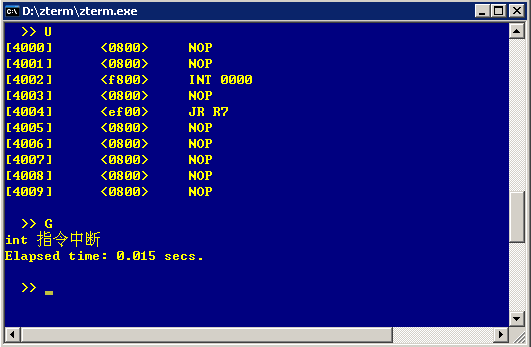
\includegraphics[width=\linewidth]{instruction_int.png}

\subsubsection{硬件中断}
使用no\_timer.bit:\\
中断测试程序如下:\\
\begin{verbatim}
LI R0 40
SLL R0 R0 0
NOP
JR R0
NOP
JR R7
NOP
\end{verbatim}
跑上面的死循环,然后拨动硬件中断开关,测试硬件中断,结果如下:\\
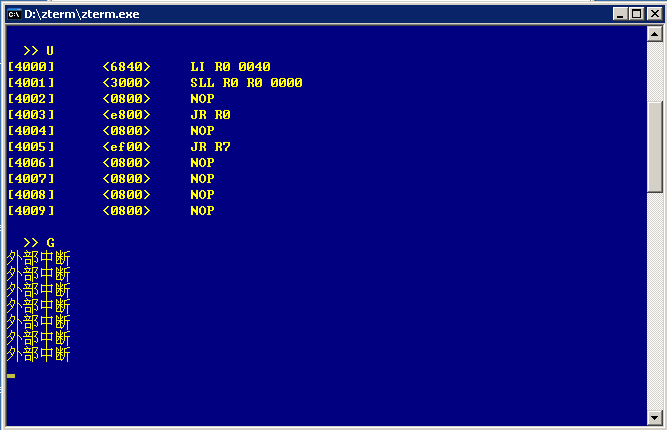
\includegraphics[width=\linewidth]{ex_int.png}

\subsubsection{时钟中断}
使用 timer\_with\_cache.bit 进行测试:\\
我们设置了时钟中断的频率为每 10000 个周期一次\\
时钟中断测试程序如下:\\
\begin{verbatim}
LI R0 40
SLL R0 R0 0
NOP
JR R0
NOP
JR R7
NOP
\end{verbatim}
即跑一个死循环,然后就会不断得有时钟中断,测试结果如下:\\
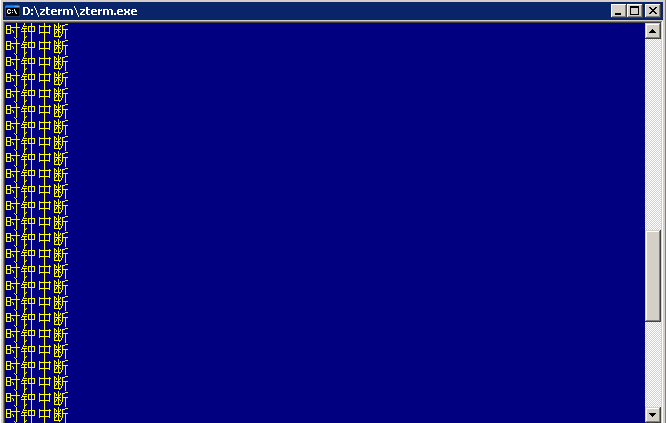
\includegraphics[width=\linewidth]{clk_int.png}

\subsection{速度测试(与多周期CPU对比)}
为了测试流水 CPU 的加速比有多高,我们还做了一个5周期的多周期 CPU ,用来对比测试。\\
多周期 CPU 速度测试\\
使用 cycle.bit ,结果如下:\\
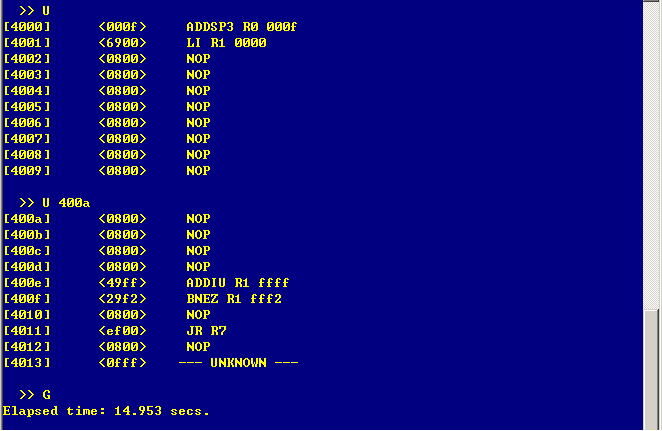
\includegraphics[width=\linewidth]{wzw_speed_long.png}
流水CPU速度测试(没有Cache)\\
使用 no\_timer.bit ,结果如下:\\
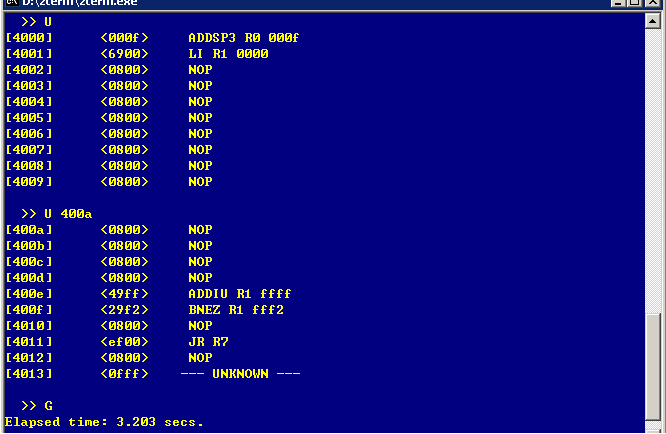
\includegraphics[width=\linewidth]{no_time_speed_long.png}
速度比:\\
$$\frac{14.953}{3.202}=4.67$$
已经比较接近5了.

\subsection{打开Cache与不打开Cache对比}
打开Cache进行测试\\
使用no\_timer\_with\_cache.bit,结果如下:\\
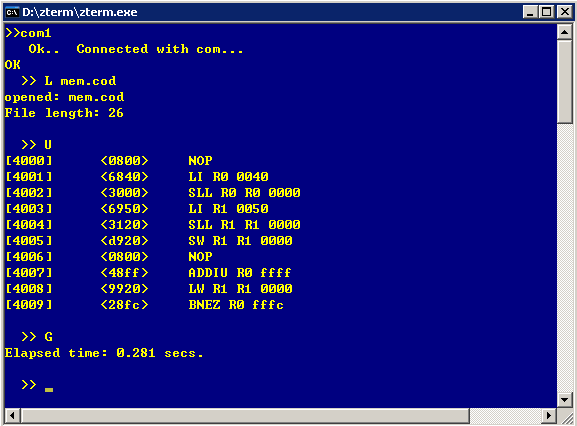
\includegraphics[width=\linewidth]{cache.png}
关闭Cache再进行测试\\
使用no\_timer.bit,结果如下:\\
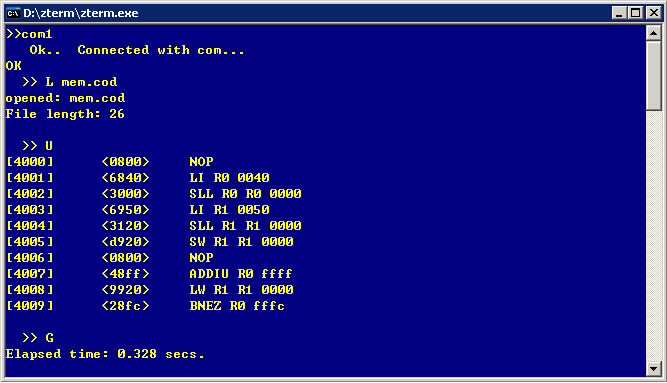
\includegraphics[width=\linewidth]{no_cache.png}

加速比:\\
$$\frac{0.328-0.281}{0.281}=16.7\%$$

\subsection{三种中断加读写内存混合测试}
使用 timer\_with\_cache.bit \\
代码如下:\\
\begin{verbatim}
LI R0 40
SLL R0 R0 0
LI R1 50
SLL R1 R1 0
SW R1 R1 0
LW R1 R1 0
INT 0
NOP
JR R0
NOP
\end{verbatim}

可以看到,在大量的指令中断中间夹杂着时钟中断,这个时候如果拨动硬件中断开关的话,还可以看到硬件中断。三种中断加上内存读写
在一起可以很好的工作,没有任何问题。证明了我们的 CPU 的鲁棒性。


\section{创新点}
\subsection{结构创新}
在前面已经提到,我们的结构设计有较大创新,一个是 MEM 和 EXE 的并行设计,另一个是 MEM,EXE 和 WB 都直接设计成组合逻辑,而把更多
直接可以完成的任务交给 ID 模块来做,这样的结构创新设计特别简单,无论是从理解上还是从编码和维护上,并且添加新的功能也
十分容易。

\subsection{控制分离}
许多组实验的设计都有 StallController ,用来控制各个模块的插气泡等过程。但是我们的设计里没有这么一个控制器,因为一方面我们
的结构创新使得我们需要做控制的地方不多,另一方面我们又采取了控制分离的模式,即控制已经分散在各个模块内部。这样的设计避免
了总控的复杂,简单明了,易于实现(一般只要加上一点判断即可)。而许多组都会因为总控过于复杂逻辑出现混乱,导致各种bug的出现。

\subsection{代码简洁}
由于设计上做了很多优化和创新,并且顶层模块连接我们又使用了 Schematic 来做,我们的代码量实际上是非常小的,如果删去为了调试
增加的冗余代码的话,我们的总代码量不到1000行。

\subsection{效率问题}
有的同学对我们的设计提出疑问:你们的 MEM 和 EXE 并行,并且 EXE , MEM , WB 都是组合逻辑,这样的 CPU 还是流水 CPU 吗?它的效率怎么样?
实际上,我们设计的时候是以课堂所学为基础,通过实践经验加上我们自己独有的创新完成的。首先,从效率上讲,流水CPU 的目标就是
通过流水技术实现指令的吞吐率,提高指令执行的速度。对于5周期的多周期 CPU 来说,一条指令的执行需要5个时钟周期,而流水 CPU 在
没有冲突的情况下可以1个时钟周期完成一条指令。我们的 CPU 也是流水的,同时也实现了一个周期一条指令的效率,因此它是一个符合
要求的流水 CPU ,只不过可能已经和经典的五阶段流水 CPU 有了一定的差异,但这恰恰体现出我们的 CPU 的创新的地方,而且它设计简单,
实现方便,无论是框架图还是代码实现都非常简单,易于理解,模块化程度高,调试容易。

\section{实验调试}
在实验的过程中,单步调试起到了巨大的作用,许多很难发现的细小的但却影响很大的 bug 都是在单步的情况下调出来的。实验箱的右上角
有48个灯,这48个灯也是 CPU 调试时唯一可以直接输出的地方,于是我们把ID阶段的两个输出接到其中的32个灯上,另外16个灯则在不同的
调试阶段给予不同的调试输出。这样,我们在单步的时候就可以看我们的输出,于是单步调式成了可能。

\section{遇到的困难}
\begin{enumerate}
\item 在刚写完最初版本的代码的时候,运行kernel程序可以向串口打印出 OK,但是之后输入U,R,D之类的 term 指令就没有任何反应了。
于是我们单步调试,发现在CPU是可以从串口接收到指令的,随后 CPU 会把收到的指令与0052(R),0044(D),0047(G)等进行比较(Kernel源代
码的216行到243行),从而确定出是什么命令。但是我们发现即使我们输入R指令,CPU 比较完了之后也没有跳转到SHOWREGS 里去,更进一步
调试后我们发现是 CMP R0 R1 之后,T寄存器的值是1,故其下一句 BTEQZ SHOWREGS 没有跳转。但是我们的代码是根据文档实现的,文档中
也确实写二者相等时T为1。后来我们问了7字班的师兄后才发现文档错了,应该相等时把 T 设为0。在我们查出这个问题后不久网络学堂
上就有了 CMP 错了的说明,悲剧,希望老师和助教布置大作业的时候确保文档的正确性,为同学们节约调试时间。

\item 上面由于文档错误的 CMP 指令改正后,我们发现各种命令仍然不能向串口输出结果,经过仔细的检查,我们发现错误出在 SW 语句上,
在 EXE 阶段处理 SW 指令的时候,我们错误得把它的立即数的位数当成了8位(实际上应该是5位),于是算出来的地址就是错的,自然串口
也不会接收到命令的输出。把这个问题解决了以后,我们的R指令就已经可以正常运行了,返回寄存器的值。

\item在调试流水 CPU 的时候,我们发现扩展内存 4001 和 4003 的内容经常会被改写。仔细测试发现,4001 和 4003 的内容在kernel运行输出 ok 后
就已经被改写成37,执行R指令或U指令后又会被改写成其他值。而且还发现用A命令写入用户代码后,第一次使用U指令读到的数据是正确
的,第二次就变成错误的了,已经被改成了其他内容。于是我们又单步调试,盯着地址线输出和数据输出,结果从头到尾一直到输出数据
到串口也没有发现任何指令去改写4001和4003的内容。于是我们陷入了困惑当中。后来,我们经过不断的调试,把改写扩展内存的范围
缩小到 kerne l初始化串口的地方,经过几番讨论,联合改变后的值为 0037 这个现象,我们觉得是在初始化串口的同时改写了扩展内存。
于是,我们对 MemController 作了一些改动,使之基本地址线和扩展地址线的 we 不同时为0,这个问题就解决了。但是实际上我们还是有
疑问,按照我们的理解,只要控制好 mio, req 等控制信号,就不应该有这个问题,所以这个问题虽然解决了,但并没有真正弄懂。

\item 在调试 Cache 的时候,我们发现总是会有数据错误的问题。这个问题的难度在于很难调试,不像前面的困难都可以单步运行找出来。
于是我们只好一遍一遍的看代码,改代码,运行测试,最后终于发现是我们在写 Cache 数据的时候 index 已经被更新了,因此写入出错。
把这个问题改掉后,Cache 模块就正常运行了。

\item FPGA有时候会死掉。在我们调试的时候,我们经常会遇到走到某一个指令的时候,所有的灯都熄灭,Reset 也无法使之复位的情况。
多次调试经验发现,FPGA 死掉多发生在 SW,ADDSP3 等语句上,但是我们一直没有找出原因所在。有时候不小心用手碰到电路的时候也会
发生死掉的问题。和助教讨论过这个问题,助教也说不准。

\item 此外我们还遇到许多诸如从串口读到大量错误数据,  指令跑飞等困难,都被我们一一克服,在此不再赘述。
\end{enumerate}

\section{实验感想}
这次实验给我们带来的感触很多。从对 CPU 结构只有一个模糊的概念到真正自己设计完成了一个流水的 CPU ,这期间,我们都学到了很多。

在此想说几点:\\

\begin{itemize}
\item 设计 CPU 虽然课本上课件上有现成的结构图,但是我们仍然根据自己的理解做了许多创新工作,这些工作不仅让我们对实现一个
流水 CPU 有了自己的理解和体会, 而且可以使我们的工作量减少,设计简洁易于理解。

\item 代码风格也很重要。由于是多人协作写代码,我们一开始就建立了 subversion 代码管理 repository, 在编写代码的时候加上了很
多 注释,特别是 ID 和 EXE 阶段,由于要对每一条指令做不同的处理,我们在每一个指令处理的地方都用注释标明指令名称,并且与指令码
对齐。这些良好的代码风格不仅大大促进了我们代码上的协作,而且给我们调试代码,理解代码都带来了极大的方便。

\item 团队协作是关键。虽然我们没有明确的分工,但是我们之间协作的很好。每次大家聚在一起开发就先讨论一下工作进度,然后一个人
负责一块就开始工作,然后过一段时间在汇总讨论。事实上这种协作模式工作得很好,虽然开发了很长时间,但是我们没有出现过任何
工作范围冲突或重叠。另外大家经常讨论,有想法时大家就立刻动手先实现一个试一试,因此也不会有争吵。就这样,我们完成了创新,
实现了我们自己设计的流水CPU。

\end{itemize}

\section{实验经验总结}

\begin{itemize}
\item 指令解码和执行模块由于指令众多,处理又各不相同,很容易出错,如果出错的话很难找出问题。我们当时就花了好多时间来找
这样的错误。因此写这两个模块的代码的时候一定要多查几遍,保证每个指令都正确解码和执行。

\item 框架结构的设计十分重要。虽然原理是一样的,架构和模块也是差不多的,但是真正实现起来却可以千差万别。从我们的经验看来,
框架结构的良好设计不仅可以使逻辑清晰,而且代码量大大减少,调试也十分简单,能节约大量的时间。

\item 单步调试十分重要。我们大部分的bug都是单步调试调出来的。而单步调试需要对指令很熟悉,同时对kernel也要很熟悉,因此
kernel代码需要多读,充分了解其原理。

\end{itemize}

\newpage

\section{附录}
\subsection{实验分工}
实际上我们许多工作都是共同完成,并没有明确的分工,在此把工作侧重点列举如下:\\
\begin{itemize}
\item 王健飞:框架设计,代码编写
\item 朱文雷:代码编写,单步调试
\item 王靖易:测试工作,代码检查
\end{itemize}

\newpage

\subsection{CPU内部指令分类表}
\begin{center}
\begin{tabular}{|c|c|c|}\hline
0&	NOP & \\\hline
% -- 2 regs
1&	ADDIU3 & \multirow{18}{*}{2 registers}\\\cline{1-2}
2&	AND&\\\cline{1-2}
3&	CMP&\\\cline{1-2}
4&	LW&\\\cline{1-2}
5&	MOVE&\\\cline{1-2}
6&	NEG&\\\cline{1-2}
7&	NOT&\\\cline{1-2}
8&	OR&\\\cline{1-2}
9&	SLL&\\\cline{1-2}
10&	SLLV&\\\cline{1-2}
11&	SLT&\\\cline{1-2}
12&	SLTU&\\\cline{1-2}
13&	SRA&\\\cline{1-2}
14&	SRAV&\\\cline{1-2}
15&	SRL&\\\cline{1-2}
16&	SRLV&\\\cline{1-2}
17&	SW&\\\cline{1-2}
18&	XOR&\\\hline
% -- 3 regs
19&	ADDU & \multirow{2}{*}{3 registers}\\\cline{1-2}
20&	SUBU&\\\hline
% -- 1 left reg
21&	ADDIU & \multirow{15}{*}{1 left register}\\\cline{1-2}
22&	ADDSP3&\\\cline{1-2}
23&	BEQZ&\\\cline{1-2}
24&	BNEZ&\\\cline{1-2}
25&	CMPI&\\\cline{1-2}
26&	JALR&\\\cline{1-2}
27&	JR&\\\cline{1-2}
28&	LI&\\\cline{1-2}
29&	LW\_SP&\\\cline{1-2}
30&	MFIH&\\\cline{1-2}
31&	MFPC&\\\cline{1-2}
32&	MTIH&\\\cline{1-2}
33&	SLTI&\\\cline{1-2}
34&	SLTUI&\\\cline{1-2}
35&	SW\_SP&\\\hline
% -- 1 right reg
36&	MTSP & 1 right register\\\hline
% -- no reg
37&	ADDSP & \multirow{7}{*}{no register} \\\cline{1-2}
38&	SW\_RS  &\\\cline{1-2}
39&	BTEQZ  &\\\cline{1-2}
40&	BTNEZ  &\\\cline{1-2}
41&	INT    &\\\cline{1-2}
42&	JRRA   &\\\cline{1-2}
43&	B      &\\\hline
\end{tabular}
\end{center}

\newpage
\subsection{指令分阶段解析表}
\begin{center}
\begin{tabular}{|c|c|c|c|c|c|c|c|c|c|c|c|c|c|c|c|}\hline
15&14&13&12&11&10&9&8&7&6&5&4&3&2&1&0\\\hline
\multicolumn{5}{|c|}5&\multicolumn{3}{|c|}3&\multicolumn{3}{|c|}3&\multicolumn{5}{|c|}5\\\hline
\multicolumn{5}{|c|}{op code}&\multicolumn{3}{|c|}{rx}&\multicolumn{3}{|c|}{ry}&\multicolumn{5}{|c|}{rz or imm}\\\hline
\end{tabular}
\end{center}

\begin{center}
\begin{longtable}{|c|c|c|c|c|c|}\hline
no.&instruction& ID               & EXE               & MEM                     & WB \\\hline
0  &   NOP     &                  &                   &                         &    \\\hline
1  &  ADDIU3   &\zcell{c}{o1=rx}  &\zcell{c}{op=ADD\\ 
								   A=i1\\
								   B=instr[3:0]\\
								   oData=Y}           &                         &\zcell{c}{
																				 reg\_addr=instr[7:5]\\
														                         write\_reg='1'}\\\hline
2  &  AND      &\zcell{c}{o1=rx\\                                                      
				o2=ry}            &\zcell{c}{op=AND\\ 
								   A=i1\\
								   B=i2\\oData=Y}     &                         &\zcell{c}{
																				 reg\_addr=instr[10:8]\\
														                         write\_reg='1'}\\\hline
3  & CMP       &\zcell{c}{o1=rx\\                                                            
				o2=ry}            &\zcell{c}{op=CMP\\ 
								   A=i1\\
								   B=i2\\oData=Y}     &                         &    \\\hline
4  & LW        &\zcell{c}{o1=rx}  &\zcell{c}{A=i1\\
							       B=instr[4:0]\\
								   oAddr=Y}           &\zcell{c}{ram\_we='1'\\
													   data\_out=data\_read}    &\zcell{c}{
																				 reg\_addr=instr[7:5]\\
														                         write\_reg='1'}\\\hline
5  & MOVE      &\zcell{c}{o2=ry}  &oData=i2           &                         &\zcell{c}{
																				 reg\_addr=instr[10:8]\\
														                         write\_reg='1'}\\\hline
6  & NEG       &\zcell{c}{o2=ry}  &\zcell{c}{op=SUB\\ 
								   A=0\\
								   B=i2\\
								   oData=Y}           &                         &\zcell{c}{
																				 reg\_addr=instr[10:8]\\
														                         write\_reg='1'}\\\hline
7  & NOT       &\zcell{c}{o2=ry}  &\zcell{c}{op=NOT\\ 
								   A=i2\\
								   oData=Y}           &                         &\zcell{c}{
																				 reg\_addr=instr[10:8]\\
														                         write\_reg='1'}\\\hline
8  & OR        &\zcell{c}{o1=rx\\                                                            
				o2=ry}            &\zcell{c}{op=OR\\
								   A=i1\\B=i2\\
								   oData=Y}           &                         &\zcell{c}{
																				 reg\_addr=instr[10:8]\\
														                         write\_reg='1'}\\\hline
9  & SLL       &\zcell{c}{o2=ry}  &\zcell{c}{op=SLL\\ 
								   A=i2\\B=imm or 8\\ 
								   oData=Y}           &                         &\zcell{c}{
																				 reg\_addr=instr[10:8]\\
														                         write\_reg='1'}\\\hline
10 & SLLV      &\zcell{c}{o1=rx\\                                                            
				o2=ry}            &\zcell{c}{op=SLL\\ 
								   A=i2\\B=i1\\
								   oData=Y}           &                         &\zcell{c}{
																				 reg\_addr=instr[7:5]\\
														                         write\_reg='1'}\\\hline
11 & SLT       &\zcell{c}{o1=rx\\                                                            
				o2=ry}            &\zcell{c}{op=LT\\ 
								   A=i1\\B=i2\\
								   oData=Y}           &                         &    \\\hline
12 & SLTU      &\zcell{c}{o1=rx\\                                                            
				o2=ry}            &\zcell{c}{op=LTU\\
								   A=i1\\B=i2\\
								   oData=Y}           &                         &    \\\hline
13 & SRA       &\zcell{c}{o2=ry}  &\zcell{c}{op=SRA\\
								   A=i2\\B=imm or 8\\
								   oData=Y}           &                         &\zcell{c}{
																				 reg\_addr=instr[10:8]\\
														                         write\_reg='1'}\\\hline
14 & SRAV      &\zcell{c}{o1=rx\\                                                            
                o2=ry}            &\zcell{c}{op=SRA\\
								   A=i2\\B=i1\\
								   oData=Y}           &                         &\zcell{c}{
																				 reg\_addr=instr[7:5]\\
														                         write\_reg='1'}\\\hline
15 & SRL       &\zcell{c}{o2=ry}  &\zcell{c}{op=SRL\\
								   A=i2\\B=imm or 8\\
								   oData=Y}           &                         &\zcell{c}{
																				 reg\_addr=instr[10:8]\\
														                         write\_reg='1'}\\\hline
16 & SRLV      &\zcell{c}{o1=rx\\                                                            
                o2=ry}            &\zcell{c}{op=SRL\\
								   A=i2\\B=i1\\
								   oData=Y}           &                         &\zcell{c}{
																				 reg\_addr=instr[7:5]\\
														                         write\_reg='1'}\\\hline
17 & SW        &\zcell{c}{o1=rx\\                                        
                o2=ry}            &\zcell{c}{op=ADD\\
								   A=i1\\
								   B=instr[4:0]\\
								   oData=i2\\
								   oAddr=Y}           &ram\_we='0'              &    \\\hline
18 & XOR       &\zcell{c}{o1=rx\\                                        
                o2=ry}            &\zcell{c}{op=XOR\\
								   A=i1\\B=i2\\
								   oData=Y}           &                         &\zcell{c}{
																				 reg\_addr=instr[10:8]\\
														                         write\_reg='1'}\\\hline
19 & ADDU      &\zcell{c}{o1=rx\\                                                            
                o2=ry}            &\zcell{c}{op=ADD\\
								   A=i1\\B=i2\\
								   oData=Y}           &                         &\zcell{c}{
																				 reg\_addr=instr[4:2]\\
														                         write\_reg='1'}\\\hline
20 & SUBU      &\zcell{c}{o1=rx\\                                                            
                o2=ry}            &\zcell{c}{op=SUB\\
								   A=i1\\B=i2\\
								   oData=Y}           &                         &\zcell{c}{
																				 reg\_addr=instr[4:2]\\
														                         write\_reg='1'}\\\hline
21 & ADDIU     &\zcell{c}{o1=rx}  &\zcell{c}{op=ADD\\
								   A=i1\\B=instr[7:0]\\
								   oData=Y}           &                         &\zcell{c}{
																				 reg\_addr=instr[10:8]\\
														                         write\_reg='1'}\\\hline
22 & ADDSP3    &o1=SP             &\zcell{c}{op=ADD\\
								   A=i1\\B=instr[7:0]\\
								   oData=Y}           &                         &\zcell{c}{
																				 reg\_addr=instr[10:8]\\
														                         write\_reg='1'}\\\hline
23 & BEQZ      &\zcell{c}{o1=rx\\
				o2=PC       }     &\zcell{c}{op=ADD\\
								   A=i2\\B=instr[7:0]\\
								   oData=Y\\
								   oAddr=i1}          &                         &    \\\hline
24 & BNEZ      &\zcell{c}{o1=rx\\
				o2=PC       }     &\zcell{c}{op=ADD\\
								   A=i2\\B=instr[7:0]\\
								   oData=Y\\
								   oAddr=i1}          &                         &    \\\hline
25 & CMPI      &\zcell{c}{o1=rx}  &\zcell{c}{op=EQ\\
								   A=i1\\B=instr[7:0]\\
								   oData=Y}           &                         &    \\\hline
26 & JALR      &\zcell{c}{o1=rx\\
				o2=PC       }     &\zcell{c}{oData=i1\\
								   oAddr=i2}          &                         &    \\\hline
27 & JR        &\zcell{c}{o1=rx}  &oData=i1           &                         &    \\\hline
28 & LI        &                  &                   &                         &\zcell{c}{
																				 reg\_addr=instr[10:8]\\
														                         write\_reg='1'}\\\hline
29 & LW\_SP    &o1=SP             &\zcell{c}{op=ADD\\
								   A=i1\\B=instr[7:0]\\
								   oAddr=Y}           &\zcell{c}{ram\_we='1'\\
													   data\_out=data\_read}    &\zcell{c}{
																				 reg\_addr=instr[10:8]\\
														                         write\_reg='1'}\\\hline
30 & MFIH      &o1=IH             &oData=i1           &                         &\zcell{c}{
																				 reg\_addr=instr[10:8]\\
														                         write\_reg='1'}\\\hline
31 & MFPC      &o1=PC             &oData=i1           &                         &\zcell{c}{
																				 reg\_addr=instr[10:8]\\
														                         write\_reg='1'}\\\hline
32 & MTIH      &\zcell{c}{o1=rx}  &oData=i1           &                         &\zcell{c}{
																				 reg\_addr=instr[10:8]\\
														                         write\_reg='1'}\\\hline
33 & SLTI      &\zcell{c}{o1=rx}  &\zcell{c}{op=LT\\
								   A=i1\\B=instr[7:0]\\
								   oData=Y}           &                         &    \\\hline
34 & SLTUI     &\zcell{c}{o1=rx}  &\zcell{c}{op=LT\\
								   A=i1\\B=instr[7:0]\\
								   oData=Y}           &                         &    \\\hline
35 & SW\_SP    &\zcell{c}{o1=rx\\
				o2=SP       }     &\zcell{c}{op=ADD\\
								   A=i2\\B=instr[7:0]\\
								   oData=i1\\
								   oAddr=Y}           &ram\_we='0'              &    \\\hline
36 & MTSP      &\zcell{c}{o1=rx}  &oData=i1           &                         &    \\\hline
37 & ADDSP     &o1=SP             &\zcell{c}{op=ADD\\
								   A=i1\\B=instr[7:0]\\
								   oData=Y}           &                         &    \\\hline
38 & SW\_RS    &\zcell{c}{o1=SP\\
				o2=RA}            &\zcell{c}{op=ADD\\
								   A=i1\\B=instr[7:0]\\
								   oData=i2\\
								   oAddr=Y}           &ram\_we='0'              &    \\\hline
39 & BTEQZ     &\zcell{c}{o1=PC\\
				o2=T}             &\zcell{c}{op=ADD\\
								   A=i1\\B=instr[7:0]\\
								   oData=Y\\
								   oAddr=i2}          &                         &    \\\hline
40 & BTNEZ     &\zcell{c}{o1=PC\\
				o2=T       }      &\zcell{c}{op=ADD\\
								   A=i1\\B=instr[7:0]\\
								   oData=Y\\
								   oAddr=i2}          &                         &    \\\hline
41 & INT       &                  &                   &ram\_we='0'              &    \\\hline
42 & JRRA      &o1=RA             &oData=i1           &                         &    \\\hline
43 & B         &o1=PC             &oData=i1           &                         &    \\\hline


\end{longtable}
\end{center}

\end{CJK}
\end{document}
